\chapter{Least Squares, the SVD and Regularization}\label{ch:least-squares}

\begin{chapterintro}
In your first physics laboratory you probably plotted a handful of measured points and drew ``the best straight line'' through them with a ruler. This chapter turns that ruler into mathematics. We ask what ``best'' should mean, derive the line that is best in the sense of least squares, and then generalize: from two coefficients (slope and intercept) to hundreds, and from straight lines to any model that is a sum of fixed functions multiplied by unknown coefficients. Along the way we meet the most useful single tool in numerical linear algebra, the singular value decomposition (SVD). It tells you exactly which combinations of coefficients your data can determine, which ones they determine badly, and which ones they cannot see at all.

The SVD also shows why fitting can go wrong. Small singular values amplify noise; problems with more coefficients than data points have infinitely many perfect fits; and a perfect fit to the data you have says nothing, by itself, about data you do not have. The cure for the first two problems is regularization (truncated SVD and ridge regression), which we derive in full. The third problem, memorization, appears here in its simplest form, a polynomial threaded through noisy points, and is taken up properly in Chapter~\ref{ch:generalization}.

Where this shows up in the paper: every iteration of the paper's potential fit is a damped least-squares problem solved with the SVD (Sec.~II~C and Appendix~A step~6 of \cite{soniR1}); the damping formula $\sigma/(\sigma^2+\lambda\sigma_1^2)$ in that step is the ridge filter of \cref{sec:least-squares-ridge}; the ridge rows of Tables~I and~II and the ridge-regularized interpolation fits of Sec.~III are ridge regression; and the sinusoidal controls B and C1 of Secs.~II~D and~IV are linear least-squares fits, one of which the paper calls ``underdetermined'' at 900 coefficients on 400 zeros.
\end{chapterintro}

\begin{prerequisites}
\item Chapter~\ref{ch:linear-algebra}: vectors in $n$ dimensions, dot (inner) product, norm, orthogonality, orthonormal bases, matrices and matrix multiplication, transpose, identity and inverse matrices, rank, solving $Ax=b$, sampling functions on a grid.
\item Chapter~\ref{ch:eigen}: eigenvalues and eigenvectors; real symmetric matrices have real eigenvalues and an orthonormal basis of eigenvectors (the spectral theorem); diagonalization.
\item Recalled briefly where used, not required: relative error and machine epsilon ($2.2\times10^{-16}$ in double precision, the relative precision of a double-precision floating-point number; Chapter~\ref{ch:asymptotics}); the cosine functions $\cos(k\pi x/L)$ on $[-L,L]$ and the prime-2 wave RE2 (Chapter~\ref{ch:fourier-series}), whose formula is restated in \cref{eq:least-squares-re2}.
\item First-year physics and calculus: derivatives, the condition $f'(x)=0$ at a smooth minimum, plotting data, the idea of measurement error.
\end{prerequisites}

%======================================================================
\section{Fitting a straight line}\label{sec:least-squares-line}

Suppose a cart rolls along a track and you record its position at four times:

\begin{table}[htbp]\centering
\caption{Positions of a cart (data for the first Sample Problem of this chapter, ``The best line for the rolling cart'').}\label{tab:least-squares-cart}
\begin{tabular}{ccccc}\toprule
time $t_i$ (s) & 0 & 1 & 2 & 3\\
position $y_i$ (m) & 1 & 3 & 4 & 4\\\bottomrule
\end{tabular}
\end{table}

You believe the cart moves at roughly constant velocity, so you want a model $y \approx c_0 + c_1 t$, where $c_0$ is the starting position (the intercept) and $c_1$ the velocity (the slope). No straight line passes through all four points. We need a rule that picks one line.

\paragraph{Residuals.} For a trial line with coefficients $(c_0,c_1)$, the \emph{residual} of point $i$ is the measured value minus the model value,
\begin{equation}
r_i = y_i - (c_0 + c_1 t_i), \qquad i=1,\dots,m,
\label{eq:least-squares-resid-line}
\end{equation}
where $m$ is the number of data points ($m=4$ here). A residual is the vertical distance from the point to the line, positive if the point lies above. A good line has small residuals. But there are $m$ residuals and we want a single number to minimize.

\paragraph{Why squares?} The least-squares rule chooses the line that minimizes the \emph{sum of squared residuals}
\begin{equation}
S(c_0,c_1) = \sum_{i=1}^{m} r_i^2 = \sum_{i=1}^m \bigl(y_i - c_0 - c_1 t_i\bigr)^2 .
\label{eq:least-squares-S-line}
\end{equation}
Four reasons make squares the standard choice. (1) Squares are never negative, so positive and negative residuals cannot cancel. (2) $S$ is a smooth function of the coefficients, so calculus finds its minimum; the sum of absolute values $\sum\abs{r_i}$ has corners where some $r_i=0$, and derivatives fail there. (3) Squaring penalizes a residual of 2 four times as much as a residual of 1, so the rule works hard to avoid large misses. (4) When measurement errors follow the Gaussian (bell-curve) distribution, least squares picks the coefficients under which the observed data are most probable (see the box below).

\begin{beyond}
\textbf{The statistical justification of least squares.} Gauss showed that if the errors in $y_i$ are independent and Gaussian with a common width, the coefficients that minimize $S$ are the ones that make the observed data most probable (maximum likelihood), and the Gauss--Markov theorem states that among all unbiased estimators that are linear in the data, least squares has the smallest variance. We do not prove these statements here; they need the probability of Chapter~\ref{ch:probability}. Proofs are in \cite{esl}. Nothing in this chapter depends on them.
\end{beyond}

\paragraph{Functions of two variables and partial derivatives.} $S$ depends on two numbers, $c_0$ and $c_1$. The \emph{partial derivative} $\partial S/\partial c_0$ is the ordinary derivative of $S$ with respect to $c_0$ while $c_1$ is held fixed (treated as a constant); $\partial S/\partial c_1$ is defined the same way with the roles swapped. At a minimum of a smooth function of two variables, both partial derivatives vanish. The reason is a one-variable argument you already know: if $(\hat c_0,\hat c_1)$ minimizes $S$, then the one-variable function $g(c_0)=S(c_0,\hat c_1)$ has a minimum at $c_0=\hat c_0$, so $g'(\hat c_0)=0$, and $g'(\hat c_0)$ is exactly $\partial S/\partial c_0$ at the minimum. The same holds for $c_1$. (Vanishing partial derivatives are necessary for a minimum; we prove in \cref{sec:least-squares-general} that for least squares they are also sufficient.)

\paragraph{Deriving the normal equations.} Differentiate \cref{eq:least-squares-S-line} term by term with the chain rule. For $c_0$, the derivative of $(y_i - c_0 - c_1 t_i)^2$ is $2(y_i - c_0 - c_1t_i)\times(-1)$:
\begin{align}
\frac{\partial S}{\partial c_0} &= \sum_{i=1}^m 2\,(y_i - c_0 - c_1 t_i)\,(-1) = -2\sum_{i=1}^m r_i, \label{eq:least-squares-dS0}\\
\frac{\partial S}{\partial c_1} &= \sum_{i=1}^m 2\,(y_i - c_0 - c_1 t_i)\,(-t_i) = -2\sum_{i=1}^m t_i r_i . \label{eq:least-squares-dS1}
\end{align}
Setting both to zero gives two conditions on the residuals of the best line:
\begin{equation}
\sum_{i=1}^m r_i = 0, \qquad \sum_{i=1}^m t_i r_i = 0.
\label{eq:least-squares-orth-line}
\end{equation}
Now expand each sum using \cref{eq:least-squares-resid-line}. The first condition reads $\sum_i y_i - \sum_i c_0 - \sum_i c_1 t_i = 0$. Since $c_0$ and $c_1$ do not depend on $i$, $\sum_i c_0 = m c_0$ and $\sum_i c_1 t_i = c_1\sum_i t_i$:
\begin{equation}
m\,c_0 + \Bigl(\sum_i t_i\Bigr)c_1 = \sum_i y_i .
\label{eq:least-squares-ne1}
\end{equation}
The second condition reads $\sum_i t_i y_i - c_0\sum_i t_i - c_1\sum_i t_i^2 = 0$, that is
\begin{equation}
\Bigl(\sum_i t_i\Bigr)c_0 + \Bigl(\sum_i t_i^2\Bigr)c_1 = \sum_i t_i y_i .
\label{eq:least-squares-ne2}
\end{equation}
\Cref{eq:least-squares-ne1,eq:least-squares-ne2} are the \emph{normal equations} for the straight line: two linear equations for two unknowns. To solve them, multiply \cref{eq:least-squares-ne1} by $\sum_i t_i$ and \cref{eq:least-squares-ne2} by $m$:
\begin{align*}
m\Bigl(\sum t_i\Bigr)c_0 + \Bigl(\sum t_i\Bigr)^2 c_1 &= \Bigl(\sum t_i\Bigr)\Bigl(\sum y_i\Bigr),\\
m\Bigl(\sum t_i\Bigr)c_0 + m\Bigl(\sum t_i^2\Bigr) c_1 &= m\sum t_iy_i .
\end{align*}
Subtract the first line from the second; the $c_0$ terms cancel:
\begin{equation}
c_1 = \frac{m\sum t_i y_i - \bigl(\sum t_i\bigr)\bigl(\sum y_i\bigr)}{m\sum t_i^2 - \bigl(\sum t_i\bigr)^2},
\qquad
c_0 = \frac{\sum y_i - c_1\sum t_i}{m}.
\label{eq:least-squares-line-sol}
\end{equation}
The second formula is \cref{eq:least-squares-ne1} solved for $c_0$. Splitting its fraction term by term shows $c_0 = \bar y - c_1\bar t$, where $\bar t = \frac1m\sum t_i$ and $\bar y=\frac1m\sum y_i$ are the averages: the best line always passes through the point of averages $(\bar t,\bar y)$.

\paragraph{When is the denominator safe?} The denominator in \cref{eq:least-squares-line-sol} equals $m\sum_i (t_i-\bar t)^2$. To see this, expand the square:
\begin{align*}
\sum_i (t_i - \bar t)^2 &= \sum_i t_i^2 - 2\bar t\sum_i t_i + m\bar t^2 \\
&= \sum_i t_i^2 - 2\Bigl(\frac1m\sum_i t_i\Bigr)\sum_i t_i + m\Bigl(\frac1m\sum_i t_i\Bigr)^2 \quad\text{(substitute } \bar t = \textstyle\frac1m\sum t_i)\\
&= \sum_i t_i^2 - 2\frac{(\sum t_i)^2}{m} + \frac{(\sum t_i)^2}{m} \quad\text{(since } m\cdot\tfrac{1}{m^2} = \tfrac1m)\\
&= \sum_i t_i^2 - \frac{(\sum t_i)^2}{m}.
\end{align*}
Multiplying by $m$ gives the denominator. A sum of squares is zero only if every term is zero, so the denominator vanishes only if all the $t_i$ are equal. That makes sense: if every measurement is taken at the same time, the data say nothing about the slope.

\begin{sample}{The best line for the rolling cart}
Find the least-squares line $y = c_0 + c_1 t$ for the data of \cref{tab:least-squares-cart}, its residuals, and the minimum value of $S$.

\textbf{Step 1: sums.} With $m=4$: $\sum t_i = 0+1+2+3 = 6$; $\sum t_i^2 = 0+1+4+9 = 14$; $\sum y_i = 1+3+4+4 = 12$; $\sum t_i y_i = 0+3+8+12 = 23$.

\textbf{Step 2: normal equations.} From \cref{eq:least-squares-ne1,eq:least-squares-ne2}:
$4c_0 + 6c_1 = 12$ and $6c_0 + 14 c_1 = 23$.

\textbf{Step 3: solve.} The first equation gives $c_0 = 3 - 1.5c_1$. Substituting into the second: $6(3-1.5c_1) + 14c_1 = 23$, so $18 + 5c_1 = 23$ and $c_1 = 1$. Then $c_0 = 3-1.5 = 1.5$.

\textbf{Step 4: residuals.} The line predicts $1.5, 2.5, 3.5, 4.5$ at $t=0,1,2,3$, so $r = (1-1.5,\,3-2.5,\,4-3.5,\,4-4.5) = (-0.5,\,0.5,\,0.5,\,-0.5)$ m.

\textbf{Step 5: check \cref{eq:least-squares-orth-line}.} $\sum r_i = 0$ and $\sum t_i r_i = 0 + 0.5 + 1.0 - 1.5 = 0$. Both hold.

\textbf{Step 6: minimum value.} $S = 4\times 0.25 = 1.0\ \mathrm{m}^2$.
\[
\boxed{\,y = 1.5\ \mathrm{m} + (1.0\ \mathrm{m/s})\,t,\qquad S_{\min} = 1.0\ \mathrm{m}^2\,}
\]
\end{sample}

\begin{figure}[htbp]\centering
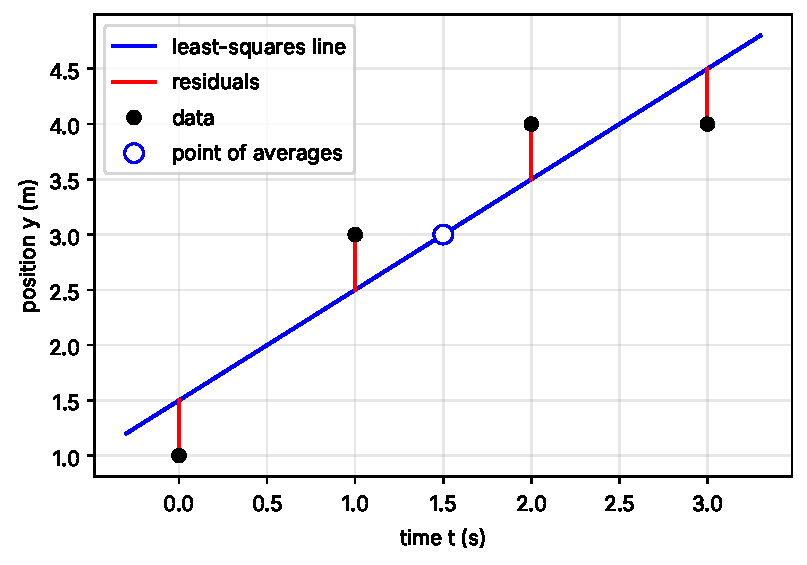
\includegraphics[width=0.85\linewidth]{figs/least-squares_line.pdf}
\caption{Least-squares line through the four cart positions of \cref{tab:least-squares-cart}. The vertical segments are the residuals $r_i$; least squares minimizes the sum of their squares. The line passes through the point of averages $(\bar t,\bar y)=(1.5\ \mathrm{s},3\ \mathrm{m})$ (open circle).}\label{fig:least-squares-line}
\end{figure}

\begin{pitfall}
Least squares as set up here measures \emph{vertical} distances, because the model treats $t$ as exact and $y$ as the noisy quantity. If you swap the roles (fit $t$ as a function of $y$), you get a different line in general. Decide first which variable carries the error.
\end{pitfall}

\begin{checkpoint}
You add $2$~m to every measured position in \cref{tab:least-squares-cart} (you moved the origin). What happens to the best-fit slope and intercept?
\end{checkpoint}
\checkanswer{The slope is unchanged and the intercept increases by 2~m. In \cref{eq:least-squares-line-sol}, $\sum y_i$ grows by $2m$ and $\sum t_iy_i$ by $2\sum t_i$, so the numerator of $c_1$ changes by $2m\sum t_i - 2m\sum t_i = 0$; then $c_0 = \bar y - c_1\bar t$ grows by $2$.}

\begin{keyideas}
\item A residual is data minus model; least squares minimizes the sum of squared residuals $S$.
\item Setting the partial derivatives of $S$ to zero gives the normal equations (\cref{eq:least-squares-ne1,eq:least-squares-ne2}), which say $\sum r_i=0$ and $\sum t_i r_i = 0$.
\item The best line passes through the point of averages; it is unique unless all $t_i$ coincide.
\end{keyideas}

%======================================================================
\section{Linear least squares in general}\label{sec:least-squares-general}

\paragraph{Linear models.} The straight line is the simplest case of a \emph{linear model}
\begin{equation}
y(t) \approx \sum_{k=1}^{M} c_k\,\phi_k(t),
\label{eq:least-squares-model}
\end{equation}
where the $\phi_k(t)$ are fixed, known \emph{basis functions} and the $c_k$ are $M$ unknown coefficients. ``Linear'' refers to the coefficients, not to $t$: the model is a sum of the $c_k$ each multiplied by something that does not depend on any $c$. Examples:
\begin{itemize}
\item the line: $M=2$, $\phi_1 = 1$, $\phi_2 = t$;
\item polynomials of degree $d$: $\phi_k = t^{k-1}$, $M = d+1$;
\item sinusoids with chosen angular frequencies $\omega_j$: $\phi = \sin(\omega_j t)$ and $\cos(\omega_j t)$ (Chapter~\ref{ch:fourier-series});
\item the cosine basis $\cos(k\pi x/L)$ on $[-L,L]$ (Chapter~\ref{ch:fourier-series}), the paper's default basis for its potential correction $\delta V(x)$.
\end{itemize}
A model such as $y = c_1\sin(c_2 t)$ is \emph{not} linear in $c_2$; fitting it is a nonlinear problem (Chapter~\ref{ch:fitting}). The paper's potential fit is nonlinear too, but it is solved by a sequence of linear problems of exactly the kind treated here (\cref{sec:least-squares-paper}).

(In this chapter the coefficient index $k$ runs from $1$ to $M$. For polynomials we will sometimes label coefficients from $0$ for convenience, and the paper labels its cosine coefficients $c_0,\dots,c_{M-1}$. Only the counting convention differs.)

\paragraph{The design matrix.} We have data $(t_i,y_i)$ for $i = 1,\dots,m$. Collect the data values into a vector $y = (y_1,\dots,y_m)$ and the coefficients into $c=(c_1,\dots,c_M)$. Define the $m\times M$ \emph{design matrix} $A$ with entries
\begin{equation}
A_{ik} = \phi_k(t_i),
\label{eq:least-squares-design}
\end{equation}
so row $i$ holds all basis functions evaluated at the $i$th data point and column $k$ holds the $k$th basis function sampled at all data points (``functions as vectors'', Chapter~\ref{ch:linear-algebra}). Then the model values at the data points are the components of the matrix-vector product $Ac$, because $(Ac)_i = \sum_k A_{ik}c_k = \sum_k c_k\phi_k(t_i)$. The \emph{residual vector} is
\begin{equation}
r = y - Ac,
\label{eq:least-squares-resid}
\end{equation}
and the least-squares problem is to minimize
\begin{equation}
S(c) = \norm{r}^2 = r^\top r = \sum_{i=1}^m \Bigl(y_i - \sum_{k=1}^M A_{ik}c_k\Bigr)^2 .
\label{eq:least-squares-S}
\end{equation}
Recall from Chapter~\ref{ch:linear-algebra} that $\norm{r}$ is the length of the vector $r$, $r^\top$ is its transpose (the vector written as a row), and $r^\top r$ is the dot product of $r$ with itself.

For the straight line, $A$ has a column of ones and a column of the $t_i$:
\[
A = \begin{pmatrix} 1 & t_1 \\ 1 & t_2\\ \vdots & \vdots\\ 1 & t_m\end{pmatrix}.
\]

\paragraph{The general normal equations.} Take the partial derivative of \cref{eq:least-squares-S} with respect to one coefficient $c_\ell$, holding the others fixed. Only the inner sum depends on $c_\ell$, and $\partial(\sum_k A_{ik}c_k)/\partial c_\ell = A_{i\ell}$ (every term with $k\neq\ell$ is a constant). By the chain rule,
\begin{align}
\frac{\partial S}{\partial c_\ell} &= \sum_{i=1}^m 2\Bigl(y_i - \sum_k A_{ik}c_k\Bigr)\,(-A_{i\ell})\nonumber\\
&= -2\sum_{i=1}^m A_{i\ell}\, r_i \nonumber\\
&= -2\,(A^\top r)_\ell . \quad\text{(definition of } A^\top:\ (A^\top)_{\ell i} = A_{i\ell})\label{eq:least-squares-grad}
\end{align}
Setting all $M$ partial derivatives to zero gives the vector equation $A^\top r = 0$. Substituting $r = y - Ac$ and moving the $c$ term to the left,
\begin{equation}
\boxed{\,A^\top A\, c = A^\top y\,}
\label{eq:least-squares-normal}
\end{equation}
These are the \emph{normal equations}: $M$ linear equations for the $M$ coefficients. The matrix $A^\top A$ is $M\times M$ with entries $(A^\top A)_{k\ell} = \sum_i \phi_k(t_i)\phi_\ell(t_i)$. For the line, $A^\top A = \begin{pmatrix} m & \sum t_i\\ \sum t_i & \sum t_i^2\end{pmatrix}$ and $A^\top y = (\sum y_i,\ \sum t_iy_i)$, which reproduces \cref{eq:least-squares-ne1,eq:least-squares-ne2}.

\paragraph{The solution really is a minimum.} A solution always exists, even when the columns of $A$ are dependent: in \cref{sec:least-squares-pinv} we construct one, $c^+$, and check that it satisfies the normal equations. Let $\hat c$ be any solution of \cref{eq:least-squares-normal} and $\hat r = y - A\hat c$ its residual, so $A^\top \hat r = 0$. For any other coefficient vector $c$,
\[
y - Ac = (y - A\hat c) + (A\hat c - Ac) = \hat r + A(\hat c - c).
\]
Take the squared length. For any vectors $a,b$, $\norm{a+b}^2 = \norm{a}^2 + 2a^\top b + \norm{b}^2$ (expand $(a+b)^\top(a+b)$). Hence
\begin{align*}
S(c) &= \norm{\hat r}^2 + 2\,\bigl(A(\hat c - c)\bigr)^\top \hat r + \norm{A(\hat c - c)}^2\\
&= \norm{\hat r}^2 + 2\,(\hat c - c)^\top A^\top \hat r + \norm{A(\hat c - c)}^2 \quad\text{(since } (AB)^\top = B^\top A^\top)\\
&= \norm{\hat r}^2 + \norm{A(\hat c - c)}^2 \quad\text{(since } A^\top \hat r = 0).
\end{align*}
So
\begin{equation}
S(c) = S(\hat c) + \norm{A(\hat c - c)}^2 \;\ge\; S(\hat c).
\label{eq:least-squares-min-identity}
\end{equation}
No coefficient vector does better than a solution of the normal equations. Equality holds exactly when $A(\hat c - c) = 0$.

\paragraph{Uniqueness.} The \emph{null space} of $A$ is the set of vectors $z$ with $Az = 0$. By \cref{eq:least-squares-min-identity}, the minimizer is unique precisely when the null space contains only $z=0$, which is the statement that the columns of $A$ are linearly independent (no nontrivial combination $\sum_k z_k a_k$ of the columns $a_k$ vanishes), that is, $\mathrm{rank}(A) = M$ (Chapter~\ref{ch:linear-algebra}). In that case $A^\top A$ is invertible. Proof: suppose $A^\top A z = 0$. Multiply on the left by $z^\top$: $0 = z^\top A^\top A z = (Az)^\top (Az) = \norm{Az}^2$, so $Az = 0$, so $z=0$ by independence. A square matrix whose only null vector is zero is invertible (Chapter~\ref{ch:linear-algebra}).

The same calculation shows that for any $z$, $z^\top A^\top A z = \norm{Az}^2 \ge 0$. A symmetric matrix with this property is called \emph{positive semidefinite}. ($A^\top A$ is symmetric because $(A^\top A)^\top = A^\top (A^\top)^\top = A^\top A$.)

\paragraph{Counting equations and unknowns.} The data give $m$ ``equations'' $y_i \approx (Ac)_i$ for $M$ unknowns.
\begin{itemize}
\item $m > M$, \emph{overdetermined}: the usual laboratory case. In general no $c$ makes $r=0$; least squares picks the best compromise.
\item $m = M$ with independent columns: $A$ is square and invertible, $c = A^{-1}y$ fits every point exactly, $S=0$.
\item $m < M$, \emph{underdetermined}: the rank of $A$ is at most $m < M$, so the columns cannot be independent and the minimizer is not unique. We will see in \cref{sec:least-squares-pinv} that there are then typically infinitely many exact fits.
\end{itemize}

\begin{checkpoint}
You fit a parabola $c_1 + c_2t + c_3t^2$ to 7 points. What are the sizes of $A$, $A^\top A$ and $A^\top y$?
\end{checkpoint}
\checkanswer{$A$ is $7\times3$; $A^\top A$ is $3\times3$; $A^\top y$ has 3 components.}

\begin{keyideas}
\item A linear model $\sum_k c_k\phi_k(t)$ evaluated at the data points is $Ac$ with design matrix $A_{ik}=\phi_k(t_i)$.
\item Least squares gives the normal equations $A^\top A c = A^\top y$, equivalently $A^\top r = 0$ (\cref{eq:least-squares-normal}).
\item Every solution of the normal equations is a global minimum (\cref{eq:least-squares-min-identity}); it is unique if and only if the columns of $A$ are independent.
\end{keyideas}

%======================================================================
\section{The geometry of least squares: projection}\label{sec:least-squares-projection}

The condition $A^\top r = 0$ has a picture. Write the columns of $A$ as vectors $a_1,\dots,a_M$ in $m$-dimensional space. Then $Ac = \sum_k c_k a_k$ is a combination of the columns. The set of all such combinations, for all possible $c$, is the \emph{column space} of $A$: a line, a plane, or a higher-dimensional flat subspace through the origin. The data vector $y$ generally does not lie in it (that is why no model fits exactly).

Component $k$ of $A^\top r$ is the dot product $a_k^\top r$. So $A^\top r = 0$ says: \emph{the residual is perpendicular to every column, and therefore to the whole column space.} The best model vector $\hat y = A\hat c$ is the foot of the perpendicular dropped from $y$ onto the column space, the \emph{orthogonal projection} of $y$. Think of a stick held above a table under the noon sun: its shadow is its projection onto the table, and the light rays (the residual) are perpendicular to the table. \Cref{eq:least-squares-min-identity} is Pythagoras' theorem: moving the model point away from the foot of the perpendicular, by $A(\hat c - c)$ within the plane, can only lengthen the distance to $y$.

Because $\hat y^\top \hat r = \hat c^\top A^\top \hat r = 0$, the data vector splits into two perpendicular pieces, and Pythagoras gives
\begin{equation}
\norm{y}^2 = \norm{\hat y}^2 + \norm{\hat r}^2 .
\label{eq:least-squares-pythagoras}
\end{equation}

\paragraph{The projection matrix.} When the columns are independent, $\hat c = (A^\top A)^{-1}A^\top y$, so
\begin{equation}
\hat y = P y,\qquad P = A(A^\top A)^{-1}A^\top .
\label{eq:least-squares-P}
\end{equation}
$P$ is an $m\times m$ matrix that sends any vector to its projection. Projecting twice changes nothing more, and the algebra confirms it: $P^2 = A(A^\top A)^{-1}(A^\top A)(A^\top A)^{-1}A^\top = A(A^\top A)^{-1}A^\top = P$.

\begin{sample}{Projecting a vector onto a plane}
Let $A$ have columns $a_1 = (1,0,1)$ and $a_2 = (0,1,1)$, and let $y = (1,2,0)$. Find the least-squares coefficients, the projection $\hat y$, the residual, and check \cref{eq:least-squares-pythagoras}.

\textbf{Step 1: normal-equation matrix.} $A^\top A = \begin{pmatrix} a_1^\top a_1 & a_1^\top a_2\\ a_2^\top a_1 & a_2^\top a_2\end{pmatrix} = \begin{pmatrix}2&1\\1&2\end{pmatrix}$.

\textbf{Step 2: right-hand side.} $A^\top y = (a_1^\top y,\ a_2^\top y) = (1+0+0,\ 0+2+0) = (1,2)$.

\textbf{Step 3: solve.} The determinant of $A^\top A$ is $2\cdot2-1\cdot1 = 3$, so $(A^\top A)^{-1} = \frac13\begin{pmatrix}2&-1\\-1&2\end{pmatrix}$ and $\hat c = \frac13(2\cdot1-1\cdot2,\ -1\cdot1+2\cdot2) = (0,1)$.

\textbf{Step 4: projection and residual.} $\hat y = 0\,a_1 + 1\,a_2 = (0,1,1)$, and $\hat r = y - \hat y = (1,1,-1)$.

\textbf{Step 5: perpendicularity.} $a_1^\top \hat r = 1+0-1 = 0$ and $a_2^\top\hat r = 0+1-1 = 0$.

\textbf{Step 6: Pythagoras.} $\norm{y}^2 = 1+4+0 = 5$; $\norm{\hat y}^2 = 0+1+1 = 2$; $\norm{\hat r}^2 = 1+1+1 = 3$; and $2+3=5$.
\[
\boxed{\,\hat c = (0,1),\quad \hat y = (0,1,1),\quad \hat r = (1,1,-1),\quad S_{\min}=3\,}
\]
\end{sample}

\begin{figure}[htbp]\centering
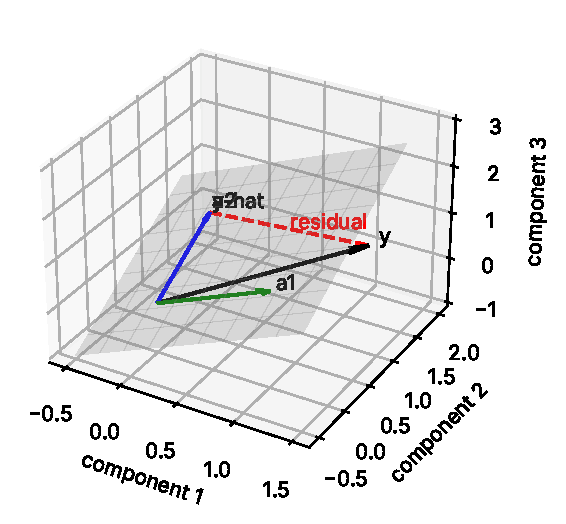
\includegraphics[width=0.85\linewidth]{figs/least-squares_projection.pdf}
\caption{The geometry of Sample Problem ``Projecting a vector onto a plane''. The shaded plane is the column space of $A$ (all combinations of $a_1=(1,0,1)$ and $a_2=(0,1,1)$). The least-squares model vector $\hat y=(0,1,1)$ is the foot of the perpendicular from the data vector $y=(1,2,0)$; the residual $\hat r = (1,1,-1)$ is perpendicular to the plane.}\label{fig:least-squares-projection}
\end{figure}

\begin{checkpoint}
In the sample problem, is the residual $\hat r$ perpendicular to the data vector $y$?
\end{checkpoint}
\checkanswer{No: $y^\top\hat r = 1+2+0 = 3 \neq 0$. The residual is perpendicular to the column space (to $a_1$, $a_2$ and $\hat y$), not to $y$.}

\begin{keyideas}
\item The model vectors $Ac$ fill the column space of $A$; least squares picks the point $\hat y$ of that space closest to $y$.
\item The residual is perpendicular to the column space; $\norm{y}^2 = \norm{\hat y}^2 + \norm{\hat r}^2$.
\item With independent columns, $\hat y = Py$ with the projection matrix $P = A(A^\top A)^{-1}A^\top$, and $P^2 = P$.
\end{keyideas}

%======================================================================
\section{The singular value decomposition}\label{sec:least-squares-svd}

The normal equations solve least squares, but they hide the information you most want: \emph{which} combinations of coefficients the data pin down well and which they pin down badly. The singular value decomposition exposes exactly this.

\paragraph{What a matrix does to a circle.} Take a $2\times2$ matrix $A$ and apply it to every unit vector $c$ (every point on the unit circle). The images $Ac$ trace out an ellipse (\cref{fig:least-squares-svd}). The ellipse has a longest axis and a shortest axis, perpendicular to each other. Their half-lengths $\sigma_1 \ge \sigma_2$ are the \emph{singular values} of $A$: the largest and smallest stretch factors the matrix applies. The unit vectors $v_1, v_2$ that land on the axes are the \emph{right singular vectors}, and the unit vectors $u_1,u_2$ along the axes are the \emph{left singular vectors}. The whole action of $A$ is then: rotate (so that $v_1, v_2$ line up with the coordinate axes), stretch each axis by $\sigma_j$, rotate again (so the axes line up with $u_1, u_2$). We now make this precise in any number of dimensions.

\paragraph{Orthogonal matrices.} A real square matrix $Q$ is \emph{orthogonal} if $Q^\top Q = I$, where $I$ is the identity matrix. Entry $(j,\ell)$ of $Q^\top Q$ is the dot product of columns $j$ and $\ell$ of $Q$, so $Q^\top Q = I$ says the columns are orthonormal (unit length, mutually perpendicular). Two consequences:
\begin{itemize}
\item $Q^\top$ is the inverse of $Q$, so also $QQ^\top = I$ (a left inverse of a square matrix is also a right inverse, Chapter~\ref{ch:linear-algebra}).
\item $Q$ preserves lengths: $\norm{Qx}^2 = (Qx)^\top(Qx) = x^\top Q^\top Q x = x^\top x = \norm{x}^2$.
\end{itemize}
Rotations and reflections are orthogonal matrices: each preserves lengths and angles, so it carries the standard unit vectors $(1,0,\dots)$, $(0,1,\dots)$, \dots, which are orthonormal, to an orthonormal set of images, and those images are exactly its columns. Recall from Chapter~\ref{ch:eigen} that the spectral theorem diagonalizes a real symmetric matrix $B$ as $B = Q D Q^\top$ with $Q$ orthogonal (columns the orthonormal eigenvectors) and $D$ diagonal (the eigenvalues).

\paragraph{Constructing the SVD.} Let $A$ be any real $m\times M$ matrix. We build its SVD in six steps.

\emph{Step 1.} The $M\times M$ matrix $A^\top A$ is symmetric (\cref{sec:least-squares-general}). By the spectral theorem it has orthonormal eigenvectors $v_1,\dots,v_M$ with real eigenvalues $\nu_1,\dots,\nu_M$, which we order so that $\nu_1\ge\nu_2\ge\cdots\ge\nu_M$. (We call these eigenvalues $\nu_j$ rather than $\lambda_j$ because $\lambda$ will soon mean a damping parameter, as in the paper.)

\emph{Step 2.} The eigenvalues are not negative: $\nu_j = \nu_j v_j^\top v_j = v_j^\top (A^\top A v_j) = \norm{Av_j}^2 \ge 0$. Define the singular values $\sigma_j = \sqrt{\nu_j}$, so $\norm{Av_j} = \sigma_j$. Let $\varrho$ be the number of strictly positive $\sigma_j$. (We write the rank as $\varrho$ because the paper uses $r$ for residuals.)

\emph{Step 3.} For $j\le\varrho$ define $u_j = Av_j/\sigma_j$. These are orthonormal:
\[
u_j^\top u_\ell = \frac{(Av_j)^\top (Av_\ell)}{\sigma_j\sigma_\ell} = \frac{v_j^\top (A^\top A v_\ell)}{\sigma_j\sigma_\ell} = \frac{\nu_\ell\, v_j^\top v_\ell}{\sigma_j\sigma_\ell} = \begin{cases}\nu_j/\sigma_j^2 = 1, & j=\ell,\\ 0, & j\neq \ell.\end{cases}
\]

Since $u_1,\dots,u_\varrho$ are $\varrho$ orthonormal vectors in $m$-dimensional space, and at most $m$ vectors there can be orthonormal (Chapter~\ref{ch:linear-algebra}), we have $\varrho\le m$; also $\varrho\le M$, since $A^\top A$ has only $M$ eigenvalues. In particular, when $M>m$ every $\sigma_j$ with $j>m$ is zero.

\emph{Step 4.} For $j>\varrho$, $\norm{Av_j} = \sigma_j = 0$, so $Av_j = 0$: these $v_j$ lie in the null space.

\emph{Step 5.} If $\varrho < m$, extend $u_1,\dots,u_\varrho$ by further unit vectors $u_{\varrho+1},\dots,u_m$ to an orthonormal basis of $m$-dimensional space (always possible, by the Gram--Schmidt procedure; see the box below).

\emph{Step 6.} Collect the vectors as columns of the orthogonal matrices $U = (u_1,\dots,u_m)$ ($m\times m$) and $V = (v_1,\dots,v_M)$ ($M\times M$), and let $\Sigma$ be the $m\times M$ matrix with $\Sigma_{jj} = \sigma_j$ for $j\le q = \min(m,M)$ and zeros elsewhere. Compare $AV$ with $U\Sigma$ column by column. Column $j$ of $AV$ is $Av_j$. Column $j$ of $U\Sigma$ is $\sigma_j u_j$ if $j\le q$ and zero if $j>q$. For $j\le\varrho$ these agree by the definition in Step 3; for $j>\varrho$ both are zero by Step 4 (either $\sigma_j=0$, or the column of $\Sigma$ is empty). So $AV = U\Sigma$. Multiply on the right by $V^\top$ and use $VV^\top = I$:
\begin{equation}
\boxed{\,A = U\,\Sigma\,V^\top\,}
\label{eq:least-squares-svd}
\end{equation}
This is the \emph{singular value decomposition}. Every real matrix has one.

\begin{beyond}
\textbf{What we took on trust.} The construction above used two results: the spectral theorem for real symmetric matrices including the case of repeated eigenvalues (stated in Chapter~\ref{ch:eigen}, with the general proof beyond this book), and the fact that any orthonormal set in $m$ dimensions can be extended to an orthonormal basis (Gram--Schmidt). Full proofs of the existence of the SVD are in \cite{strang} and \cite{trefethen}. For complex matrices the same theorem holds with $U$ and $V$ unitary and $V^\top$ replaced by the conjugate transpose $V^\dagger$. Numerically the SVD is never computed by forming $A^\top A$ (that loses accuracy, \cref{sec:least-squares-cond}); library routines use a reduction to bidiagonal form (Golub--Kahan) at a cost proportional to $mM^2$ for $m\ge M$ \cite{trefethen,nr}.
\end{beyond}

\paragraph{The outer-product form.} Write out $U\Sigma V^\top$. The product $U\Sigma$ has columns $\sigma_1u_1,\dots,\sigma_q u_q$ followed by zero columns, and multiplying a matrix of columns by $V^\top$ (whose rows are $v_j^\top$) gives the sum of each column times the corresponding row. Dropping the zero terms,
\begin{equation}
A = \sum_{j=1}^{\varrho} \sigma_j\, u_j\, v_j^\top .
\label{eq:least-squares-outer}
\end{equation}
Each term $u_jv_j^\top$ is an $m\times M$ matrix of rank one. Applied to a vector,
\begin{equation}
Ac = \sum_{j=1}^\varrho \sigma_j\,(v_j^\top c)\,u_j :
\label{eq:least-squares-action}
\end{equation}
measure the component of $c$ along each $v_j$, multiply it by $\sigma_j$, and lay it down along $u_j$. That is the rotate, stretch, rotate picture in words.

\paragraph{What the SVD tells you.}
\begin{itemize}
\item The rank of $A$ is $\varrho$, the number of nonzero singular values; the column space is spanned by $u_1,\dots,u_\varrho$ (by \cref{eq:least-squares-action}, every $Ac$ is a combination of them, and each $u_j = A(v_j/\sigma_j)$ is in it).
\item The null space is spanned by $v_{\varrho+1},\dots,v_M$. A coefficient change along these directions changes nothing at the data points.
\item A coefficient change along $v_j$ with small $\sigma_j$ changes the model values only a little. The data barely ``see'' these directions, and, as we shall see, noise in the data pushes the fitted coefficients far along them.
\item The vectors $u_j$ are eigenvectors of $AA^\top$ with the same eigenvalues $\sigma_j^2$: $AA^\top u_j = AA^\top A v_j/\sigma_j = A(\sigma_j^2 v_j)/\sigma_j = \sigma_j^2 u_j$.
\end{itemize}
The singular values are unique: they are the square roots of the eigenvalues of $A^\top A$, and those eigenvalues are fixed by $A$ (they are the roots of the characteristic polynomial of $A^\top A$). When the \emph{nonzero} $\sigma_j$ are distinct, each $\sigma_j^2$ is a simple eigenvalue of the symmetric matrix $A^\top A$, so its unit eigenvector $v_j$ is unique up to sign, and $u_j = Av_j/\sigma_j$ is then fixed by $v_j$ (flipping the sign of both $u_j$ and $v_j$ leaves \cref{eq:least-squares-outer} unchanged). Singular vectors belonging to a repeated singular value, or to $\sigma_j = 0$ (the null directions), are not unique: any orthonormal basis of the corresponding space will do.

For $m\ge M$ one often keeps only the first $M$ columns of $U$; this \emph{thin SVD} $A = U_M\Sigma_M V^\top$ with $\Sigma_M$ square diagonal contains everything in \cref{eq:least-squares-outer}.

\begin{sample}{SVD of a $2\times2$ matrix by hand}
Find the SVD of $A = \begin{pmatrix}3&0\\4&5\end{pmatrix}$, and verify the outer-product form.

\textbf{Step 1: form $A^\top A$.} $A^\top = \begin{pmatrix}3&4\\0&5\end{pmatrix}$, so $A^\top A = \begin{pmatrix}9+16 & 0+20\\ 0+20 & 0+25\end{pmatrix} = \begin{pmatrix}25&20\\20&25\end{pmatrix}$.

\textbf{Step 2: eigenvalues.} The characteristic polynomial (Chapter~\ref{ch:eigen}) is $(25-\nu)^2 - 400 = 0$, so $25-\nu = \pm20$, giving $\nu_1 = 45$, $\nu_2 = 5$. The singular values are $\sigma_1 = \sqrt{45} = 3\sqrt5 \approx 6.708$ and $\sigma_2 = \sqrt5 \approx 2.236$.

\textbf{Step 3: right singular vectors.} For $\nu=45$: $(25-45)x + 20 y = 0$ gives $x=y$, so $v_1 = (1,1)/\sqrt2$. For $\nu = 5$: $20x + 20y = 0$, so $v_2 = (1,-1)/\sqrt2$.

\textbf{Step 4: left singular vectors.} $Av_1 = (3,\,9)/\sqrt2$, so $u_1 = Av_1/\sigma_1 = (3,9)/(\sqrt2\cdot3\sqrt5) = (1,3)/\sqrt{10}$. $Av_2 = (3,\,4-5)/\sqrt2 = (3,-1)/\sqrt2$, so $u_2 = (3,-1)/(\sqrt2\sqrt5) = (3,-1)/\sqrt{10}$. Check: $u_1^\top u_2 = (3-3)/10 = 0$.

\textbf{Step 5: outer products.} $\sigma_1 u_1v_1^\top = \frac{3\sqrt5}{\sqrt{20}}\begin{pmatrix}1&1\\3&3\end{pmatrix} = \frac32\begin{pmatrix}1&1\\3&3\end{pmatrix}$ (since $\sqrt{20}=2\sqrt5$) and $\sigma_2u_2v_2^\top = \frac{\sqrt5}{\sqrt{20}}\begin{pmatrix}3&-3\\-1&1\end{pmatrix} = \frac12\begin{pmatrix}3&-3\\-1&1\end{pmatrix}$. Their sum is $\begin{pmatrix}1.5+1.5 & 1.5-1.5\\ 4.5-0.5 & 4.5+0.5\end{pmatrix} = \begin{pmatrix}3&0\\4&5\end{pmatrix} = A$.

\textbf{Step 6: a check.} For a square matrix, $\abs{\det A} = \sigma_1\sigma_2$ (the determinants of $U$ and $V$ are $\pm1$, Chapter~\ref{ch:linear-algebra}). Here $\det A = 15$ and $\sigma_1\sigma_2 = 3\sqrt5\cdot\sqrt5 = 15$.
\[
\boxed{\,\sigma_1 = 3\sqrt5\approx 6.708,\ \sigma_2 = \sqrt5\approx2.236;\ v_{1,2} = \tfrac{(1,\pm1)}{\sqrt2},\ u_1 = \tfrac{(1,3)}{\sqrt{10}},\ u_2=\tfrac{(3,-1)}{\sqrt{10}}\,}
\]
\end{sample}

\begin{figure}[htbp]\centering
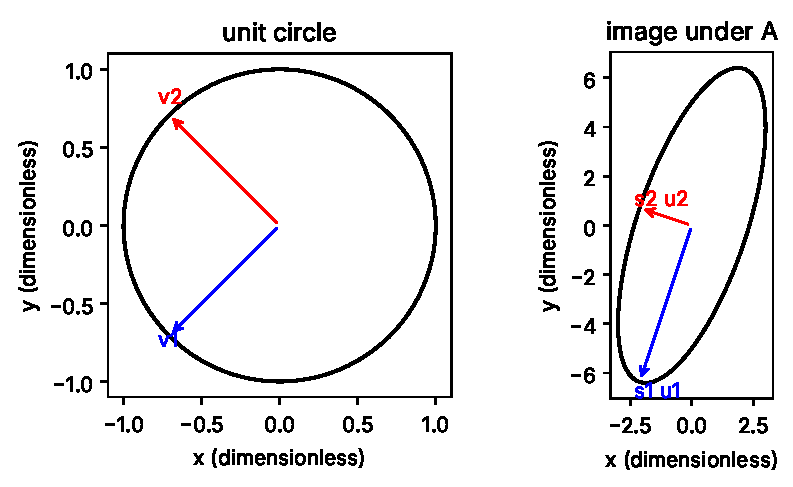
\includegraphics[width=0.95\linewidth]{figs/least-squares_svd.pdf}
\caption{The SVD as rotate, stretch, rotate, for $A=\begin{pmatrix}3&0\\4&5\end{pmatrix}$. Left: the unit circle and the right singular vectors $v_1,v_2$. Right: the image of the circle under $A$ is an ellipse whose semi-axes are $\sigma_1u_1$ and $\sigma_2u_2$, with $\sigma_1 = 3\sqrt5$ and $\sigma_2=\sqrt5$. Both axes are dimensionless.}\label{fig:least-squares-svd}
\end{figure}

\begin{pycode}
import numpy as np
A = np.array([[3.0, 0.0],
              [4.0, 5.0]])
U, s, Vh = np.linalg.svd(A)    # s holds sigma_1 >= sigma_2
print(s)                       # [6.70820393 2.23606798]
V = Vh.T                       # numpy returns V transposed!
print(np.allclose(U @ np.diag(s) @ Vh, A))   # True
print(s[0] * s[1], np.linalg.det(A))        # both 15 (det up to sign)
\end{pycode}

\begin{pitfall}
\texttt{numpy.linalg.svd} returns $V^\top$ (often called \texttt{Vh}), not $V$. The right singular vectors are the \emph{rows} of \texttt{Vh}, or the columns of \texttt{Vh.T}. Mixing these up gives wrong answers that still have the right shapes, so no error message warns you.
\end{pitfall}

\begin{checkpoint}
What are the singular values of (a) a $3\times 3$ orthogonal matrix $Q$, (b) $\mathrm{diag}(3,-2)$?
\end{checkpoint}
\checkanswer{(a) All three equal 1: $Q^\top Q = I$ has every eigenvalue 1. (b) $3$ and $2$: $A^\top A = \mathrm{diag}(9,4)$. The minus sign is absorbed into $U$ (take $u_2 = (0,-1)$).}

\begin{keyideas}
\item Every real matrix factors as $A = U\Sigma V^\top$ (\cref{eq:least-squares-svd}): orthogonal $U$, $V$ and nonnegative singular values $\sigma_1\ge\sigma_2\ge\cdots$ on the diagonal of $\Sigma$.
\item $\sigma_j^2$ are the eigenvalues of $A^\top A$; $v_j$ its eigenvectors; $u_j = Av_j/\sigma_j$.
\item $A = \sum_j\sigma_ju_jv_j^\top$: the direction $v_j$ in coefficient space produces the pattern $u_j$ in data space with gain $\sigma_j$. Zero singular values mark directions the data cannot see.
\end{keyideas}

%======================================================================
\section{Solving least squares with the SVD: the pseudo-inverse}\label{sec:least-squares-pinv}

\paragraph{Diagonalizing the problem.} Insert $A = U\Sigma V^\top$ into the objective. Because $U^\top$ is orthogonal it preserves lengths, so
\[
S(c) = \norm{y - Ac}^2 = \norm{U^\top(y - U\Sigma V^\top c)}^2 = \norm{U^\top y - \Sigma V^\top c}^2 ,
\]
using $U^\top U = I$. Introduce new coordinates: $\beta = U^\top y$ (so $\beta_j = u_j^\top y$, the component of the data along pattern $u_j$) and $\xi = V^\top c$ (so $\xi_j = v_j^\top c$, the component of the coefficients along direction $v_j$). Since $V$ is orthogonal, $c = V\xi = \sum_j \xi_j v_j$ and $\norm{c} = \norm{\xi}$. The vector $\Sigma\xi$ has components $\sigma_j\xi_j$ for $j\le q$ and zeros below. Hence, using $\sigma_j = 0$ for $\varrho<j\le q$,
\begin{equation}
S = \sum_{j=1}^{\varrho} (\beta_j - \sigma_j\xi_j)^2 + \sum_{j=\varrho+1}^{m}\beta_j^2 .
\label{eq:least-squares-S-diag}
\end{equation}
In these coordinates the problem has fallen apart into independent one-variable pieces.
\begin{itemize}
\item Each term in the first sum is minimized (made zero) by $\xi_j = \beta_j/\sigma_j$, for $j\le\varrho$.
\item The second sum does not depend on $c$ at all: it is the part of the data that no model can reach. So $S_{\min} = \sum_{j>\varrho}\beta_j^2$.
\item The coefficients $\xi_j$ with $\varrho < j\le M$ do not appear in $S$. They are completely undetermined by the data.
\end{itemize}

\paragraph{The minimum-norm solution.} Every vector $c = \sum_{j\le\varrho}(\beta_j/\sigma_j)v_j + \sum_{j>\varrho}\xi_jv_j$, with any values of the free $\xi_j$, minimizes $S$. Its squared length is $\norm{c}^2 = \sum_{j\le\varrho}(\beta_j/\sigma_j)^2 + \sum_{j>\varrho}\xi_j^2$, smallest when every free $\xi_j$ is zero. The shortest least-squares solution is therefore
\begin{equation}
\boxed{\,c^{+} = \sum_{j=1}^{\varrho} \frac{u_j^\top y}{\sigma_j}\, v_j = A^{+}y,\qquad A^{+} = V\Sigma^{+}U^\top\,}
\label{eq:least-squares-pinv-sol}
\end{equation}
where $\Sigma^+$ is the $M\times m$ matrix with $1/\sigma_j$ in position $(j,j)$ for $j\le\varrho$ and zeros elsewhere. $A^+$ is the (Moore--Penrose) \emph{pseudo-inverse} of $A$. Read \cref{eq:least-squares-pinv-sol} as a recipe: project the data onto each pattern $u_j$, divide by the gain $\sigma_j$, and build the coefficients from the directions $v_j$.

\paragraph{The pseudo-inverse solves the normal equations.} Using $A^\top = V\Sigma^\top U^\top$, $A^\top Ac^+ = V\Sigma^\top U^\top U\Sigma V^\top V\Sigma^+U^\top y$. With $U^\top U = I$ and $V^\top V = I$ this is $V(\Sigma^\top\Sigma\Sigma^+)U^\top y$. The $M\times m$ matrix $\Sigma^\top\Sigma\Sigma^+$ has entry $\sigma_j^2\cdot(1/\sigma_j) = \sigma_j$ in position $(j,j)$ for $j\le\varrho$ and zeros elsewhere. That is exactly $\Sigma^\top$, whose diagonal entries with $j>\varrho$ are zero. Hence $A^\top Ac^+ = V\Sigma^\top U^\top y = A^\top y$: the normal equations always have at least one solution, as promised in \cref{sec:least-squares-general}.

\paragraph{Agreement with the normal equations.} If the columns of $A$ are independent ($\varrho = M\le m$), then $c^+$ equals $(A^\top A)^{-1}A^\top y$. Proof: $A^\top A = V\Sigma^\top U^\top U\Sigma V^\top = V(\Sigma^\top\Sigma)V^\top$, where $\Sigma^\top\Sigma = \mathrm{diag}(\sigma_1^2,\dots,\sigma_M^2)$ is invertible. Its inverse is $V(\Sigma^\top\Sigma)^{-1}V^\top$ (multiply out and use $V^\top V = I$). Then
\[
(A^\top A)^{-1}A^\top = V(\Sigma^\top\Sigma)^{-1}V^\top\,V\Sigma^\top U^\top = V(\Sigma^\top\Sigma)^{-1}\Sigma^\top U^\top = V\Sigma^+U^\top ,
\]
because $(\Sigma^\top\Sigma)^{-1}\Sigma^\top$ has diagonal entries $\sigma_j/\sigma_j^2 = 1/\sigma_j$. If $A$ is square and invertible, $A^+ = A^{-1}$.

\paragraph{Underdetermined problems: infinitely many exact fits.} Suppose $m<M$ and the rank is as large as possible, $\varrho = m$ (the rows are independent). Then the second sum in \cref{eq:least-squares-S-diag} is empty, $S_{\min}=0$, and every point is fitted exactly. The free directions $v_{m+1},\dots,v_M$ span a null space of dimension $M - m$. Any vector $z$ in it can be added to $c^+$ without changing a single model value, so
\begin{equation}
c = c^+ + z,\qquad Az = 0,
\label{eq:least-squares-general-sol}
\end{equation}
is an exact fit for every $z$: infinitely many perfect fits. In general (any rank) the null space has dimension $M - \varrho \ge M - m$. Because $c^+$ is built from $v_1,\dots,v_\varrho$ and $z$ from $v_{\varrho+1},\dots,v_M$, the two are perpendicular and $\norm{c}^2 = \norm{c^+}^2 + \norm{z}^2$: the minimum-norm solution does nothing at all in the directions the data cannot see.

\begin{sample}{One equation, two unknowns}
Find all exact solutions of $c_1 + 2c_2 = 5$ and the minimum-norm one, first directly and then from the SVD.

\textbf{Step 1: all solutions.} Here $A = (1\ \ 2)$ is $1\times 2$. Setting $c_2 = s$ gives $c_1 = 5 - 2s$, so the solutions are $c = (5-2s,\ s)$, a whole line.

\textbf{Step 2: shortest.} $\norm{c}^2 = (5-2s)^2 + s^2 = 25 - 20s + 5s^2$. Its derivative $-20 + 10s$ vanishes at $s = 2$, giving $c = (1,2)$ with $\norm{c}^2 = 5$.

\textbf{Step 3: SVD.} $A^\top A = \begin{pmatrix}1&2\\2&4\end{pmatrix}$ has eigenvalues $5$ and $0$; $\sigma_1 = \sqrt5$, $v_1 = (1,2)/\sqrt5$, $u_1 = Av_1/\sigma_1 = (5/\sqrt5)/\sqrt5 = 1$. The null direction is $v_2 = (2,-1)/\sqrt5$.

\textbf{Step 4: pseudo-inverse solution.} $c^+ = (u_1 y/\sigma_1)\,v_1 = (5/\sqrt5)(1,2)/\sqrt5 = (1,2)$, as in Step 2. Every other exact solution is $(1,2) + s'(2,-1)$, a null vector added; for example $(5,0)$ has $s'=2$ and norm $5 > \sqrt5$.
\[
\boxed{\,c^+ = (1,2),\quad \norm{c^+}=\sqrt5\approx2.236\,}
\]
\end{sample}

\begin{pycode}
import numpy as np
A = np.array([[1.0, 2.0]])
y = np.array([5.0])
c_lstsq = np.linalg.lstsq(A, y, rcond=None)[0]  # returns the min-norm solution
c_pinv  = np.linalg.pinv(A) @ y                  # same thing via A^+
print(c_lstsq, c_pinv)                           # [1. 2.] [1. 2.]
\end{pycode}

\begin{checkpoint}
A model has $M=5$ coefficients and you have $m=3$ data points. At most how many nonzero singular values does $A$ have, and at least how large is its null space?
\end{checkpoint}
\checkanswer{At most $\min(3,5)=3$ nonzero singular values, so the rank is at most 3 and the null space has dimension at least $5-3 = 2$.}

\begin{keyideas}
\item In SVD coordinates, least squares splits into independent pieces: $\xi_j = \beta_j/\sigma_j$ for $\sigma_j>0$; the rest are free (\cref{eq:least-squares-S-diag}).
\item The pseudo-inverse $A^+ = V\Sigma^+U^\top$ gives the shortest least-squares solution (\cref{eq:least-squares-pinv-sol}); with independent columns it equals $(A^\top A)^{-1}A^\top$.
\item With more coefficients than independent data, there are infinitely many exact fits, differing by null-space vectors (\cref{eq:least-squares-general-sol}).
\end{keyideas}

%======================================================================
\section{Condition number and noise amplification}\label{sec:least-squares-cond}

\paragraph{Gains are bounded by the singular values.} For any coefficient vector $c$ with SVD coordinates $\xi = V^\top c$, \cref{eq:least-squares-action} and the orthonormality of the $u_j$ give $\norm{Ac}^2 = \sum_{j\le\varrho}\sigma_j^2\xi_j^2$. Replacing every $\sigma_j$ by the largest one can only increase the sum, so $\norm{Ac}^2\le\sigma_1^2\sum_j\xi_j^2 = \sigma_1^2\norm{c}^2$:
\begin{equation}
\norm{Ac}\le\sigma_1\norm{c}.
\label{eq:least-squares-upper}
\end{equation}
If $A$ is square ($m = M$) and invertible, all $\sigma_j>0$ (a zero $\sigma_j$ would give $Av_j = 0$ with $v_j\neq0$). Then $A^{-1} = V\Sigma^{-1}U^\top$; check: $(V\Sigma^{-1}U^\top)(U\Sigma V^\top) = V\Sigma^{-1}\Sigma V^\top = VV^\top = I$. This product has the form orthogonal matrix times diagonal matrix with positive entries $1/\sigma_j$ times the transpose of an orthogonal matrix, so after reordering the entries into decreasing order (and the columns of $V$ and $U$ with them) it is an SVD of $A^{-1}$. Its singular values are the $1/\sigma_j$, the largest being $1/\sigma_M$. Applying \cref{eq:least-squares-upper} to $A^{-1}$:
\begin{equation}
\norm{A^{-1}w}\le\frac{\norm{w}}{\sigma_M}.
\label{eq:least-squares-lower}
\end{equation}

\paragraph{The condition number.} The \emph{condition number} of a square invertible matrix is the ratio of the largest to the smallest stretch,
\begin{equation}
\kappa(A) = \frac{\sigma_1}{\sigma_M}\ \ge 1 .
\label{eq:least-squares-kappa}
\end{equation}
For a rectangular matrix with independent columns we use the same ratio $\sigma_1/\sigma_M$. Now suppose $Ac = y$ and the data change by $\delta y$, so the solution changes by $\delta c$ with $A(c+\delta c) = y + \delta y$. Subtracting, $A\,\delta c = \delta y$, so $\delta c = A^{-1}\delta y$ and by \cref{eq:least-squares-lower} $\norm{\delta c}\le\norm{\delta y}/\sigma_M$. Also, by \cref{eq:least-squares-upper}, $\norm{y} = \norm{Ac}\le\sigma_1\norm{c}$, so $1/\norm{c}\le\sigma_1/\norm{y}$. Multiplying the two inequalities,
\begin{equation}
\frac{\norm{\delta c}}{\norm{c}}\ \le\ \kappa(A)\,\frac{\norm{\delta y}}{\norm{y}} .
\label{eq:least-squares-cond-bound}
\end{equation}
A relative error in the data can be magnified by up to $\kappa$ in the solution. A matrix with large $\kappa$ is called \emph{ill-conditioned}.

\begin{sample}{An ill-conditioned pair of equations}
Solve $c_1 + c_2 = 2$, $c_1 + 1.001c_2 = 2.001$; then change the second right-hand side to $2.002$ and solve again. Compare the relative changes with the bound \cref{eq:least-squares-cond-bound}.

\textbf{Step 1: original solution.} Subtracting the equations, $0.001c_2 = 0.001$, so $c_2 = 1$ and $c_1 = 1$: $c = (1,1)$.

\textbf{Step 2: perturbed solution.} Now $0.001 c_2 = 0.002$, so $c_2 = 2$ and $c_1 = 0$: $c = (0,2)$. The data changed in the fourth significant figure; the solution changed completely.

\textbf{Step 3: relative changes.} $\norm{\delta y} = 0.001$ and $\norm{y} = \sqrt{2^2 + 2.001^2} = \sqrt{8.004001}\approx 2.8291$, so $\norm{\delta y}/\norm{y}\approx3.535\times10^{-4}$. $\norm{\delta c} = \norm{(-1,1)} = \sqrt2$ and $\norm{c} = \sqrt2$, so $\norm{\delta c}/\norm{c} = 1$. The amplification is $1/(3.535\times10^{-4})\approx 2829$.

\textbf{Step 4: condition number.} $A = \begin{pmatrix}1&1\\1&1.001\end{pmatrix}$ is symmetric with positive eigenvalues, so its singular values equal its eigenvalues. (Reason: if $B$ is symmetric with eigenvalues $\beta_j\ge0$ and orthonormal eigenvectors $q_j$, then $B^\top B = B^2$ and $B^2q_j = \beta_j^2q_j$, so the eigenvalues of $B^\top B$ are $\beta_j^2$ and the singular values are $\sqrt{\beta_j^2} = \beta_j$.) The trace is $2.001$ and the determinant $0.001$, so the eigenvalues are $\frac12\bigl(2.001\pm\sqrt{2.001^2 - 0.004}\bigr)$, i.e.\ $\sigma_1\approx2.0005$ and $\sigma_2 = 0.001/\sigma_1\approx 4.999\times10^{-4}$. Then $\kappa = \sigma_1/\sigma_2 = \sigma_1^2/0.001\approx 4002$.

\textbf{Step 5: compare.} The observed amplification, about $2829$, is below the bound $\kappa\approx4002$, as \cref{eq:least-squares-cond-bound} requires.
\[
\boxed{\,\kappa\approx 4.0\times10^3,\qquad \text{observed amplification}\approx 2.8\times10^3\,}
\]
\end{sample}

\paragraph{Noise amplification in least squares.} Real data contain noise: $y = y_{\rm true} + e$, where $e$ is the vector of measurement errors. Insert this into \cref{eq:least-squares-pinv-sol}:
\begin{equation}
c^+ = \sum_{j=1}^{\varrho}\frac{u_j^\top y_{\rm true}}{\sigma_j}v_j \;+\; \sum_{j=1}^{\varrho}\frac{u_j^\top e}{\sigma_j}v_j .
\label{eq:least-squares-noise}
\end{equation}
The first sum is what we want. The second is the noise, and each of its components is divided by $\sigma_j$. What follows is a heuristic, true in many problems but not in all, and we do not prove it. Measurement noise usually has comparable components along every pattern $u_j$ (it has no reason to prefer one), while a smooth true signal often has components $u_j^\top y_{\rm true}$ that become small for the patterns with small $\sigma_j$, which in many problems are the rapidly wiggling ones. Whether this holds must be checked problem by problem. When it does, for those $j$ the noise term dominates and is magnified by the large factor $1/\sigma_j$. The fitted coefficients then contain large, meaningless excursions along the poorly seen directions $v_j$. This is the precise sense in which ``small singular values amplify noise''.

\paragraph{Floating point and the normal equations.} Even exact data carry rounding error of relative size about machine epsilon, $2.2\times10^{-16}$ in double precision (Chapter~\ref{ch:asymptotics}). By \cref{eq:least-squares-cond-bound}, a useful rule of thumb is that you can lose up to about $\log_{10}\kappa$ significant digits. Forming the normal equations makes things worse: the singular values of the symmetric positive semidefinite matrix $A^\top A$ are its eigenvalues $\sigma_j^2$ (by the remark in Step~4 of the sample above), so
\begin{equation}
\kappa(A^\top A) = \frac{\sigma_1^2}{\sigma_M^2} = \kappa(A)^2 .
\label{eq:least-squares-kappa2}
\end{equation}
A problem with $\kappa(A) = 10^8$ is solvable with about eight good digits by an SVD-based (or QR-based) method, but $\kappa(A^\top A) = 10^{16}$ wipes out essentially every digit of a double-precision normal-equations solution. Library routines such as \texttt{numpy.linalg.lstsq} therefore work with the SVD, and the paper's update (Appendix~A step~6) is also written in SVD form, which in addition makes the damping filter explicit.

\begin{pitfall}
The normal equations are the right way to \emph{derive} least squares and the wrong way to \emph{compute} it when $A$ is ill-conditioned. Forming $A^\top A$ squares the condition number \cref{eq:least-squares-kappa2}. Use \texttt{numpy.linalg.lstsq} or an explicit SVD.
\end{pitfall}

\begin{checkpoint}
A least-squares problem has $\kappa(A)=10^5$. Roughly how many significant digits can you expect from an SVD solution in double precision, and from the normal equations?
\end{checkpoint}
\checkanswer{Double precision carries about 16 digits. Losing about 5 leaves roughly 11 with the SVD; the normal equations have $\kappa = 10^{10}$ and leave roughly 6. These are rule-of-thumb estimates, not guarantees.}

\begin{keyideas}
\item $\kappa = \sigma_1/\sigma_M$ bounds how much relative data errors are magnified (\cref{eq:least-squares-cond-bound}).
\item In the least-squares solution the noise along pattern $u_j$ is divided by $\sigma_j$ (\cref{eq:least-squares-noise}); small singular values amplify noise.
\item $\kappa(A^\top A) = \kappa(A)^2$, so compute with the SVD, not the normal equations.
\end{keyideas}

%======================================================================
\section{Truncated SVD}\label{sec:least-squares-tsvd}

The simplest defense against noise amplification is to ignore the directions that the data see badly. Keep only the $J$ largest singular values:
\begin{equation}
c^{(J)} = \sum_{j=1}^{J}\frac{u_j^\top y}{\sigma_j}v_j ,\qquad J\le\varrho .
\label{eq:least-squares-tsvd}
\end{equation}
This is the \emph{truncated SVD} solution. It is convenient to write every such solution in one form,
\begin{equation}
c = \sum_{j=1}^\varrho f_j\,\frac{u_j^\top y}{\sigma_j}\,v_j ,
\label{eq:least-squares-filter-form}
\end{equation}
where the numbers $f_j$ are \emph{filter factors}. The pseudo-inverse has $f_j = 1$ for every $j$; the truncated SVD has $f_j = 1$ for $j\le J$ and $f_j = 0$ for $j>J$.

Truncation is a trade. It removes the amplified noise in the discarded directions, but it also discards whatever true signal lay along them: the truncated solution is systematically pulled toward zero in those directions (statisticians call this \emph{bias}, and the noise-driven scatter \emph{variance}; see Chapter~\ref{ch:generalization}). A sensible cut keeps the components with $\sigma_j$ large enough that $\abs{u_j^\top y_{\rm true}}$ stands above the noise; finding that cut requires some knowledge of the noise level or a validation test.

\begin{checkpoint}
What truncated-SVD solution do you get with $J = \varrho$? With $J = 0$?
\end{checkpoint}
\checkanswer{$J=\varrho$ keeps every nonzero singular value: the pseudo-inverse solution $c^+$. $J=0$ keeps nothing: $c = 0$, the model with no fitted correction at all.}

\begin{keyideas}
\item Regularized solutions have the form (\cref{eq:least-squares-filter-form}) with filter factors $0\le f_j\le1$.
\item The truncated SVD uses a sharp cutoff: $f_j = 1$ for the $J$ largest $\sigma_j$, else $0$.
\item Truncation trades noise (variance) for systematic shrinkage toward zero (bias).
\end{keyideas}

%======================================================================
\section{Ridge regularization}\label{sec:least-squares-ridge}

A sharp cutoff is crude: a singular value just above the cut is kept whole, one just below is thrown away. Ridge regularization (also called Tikhonov regularization) replaces the step with a smooth filter.

\paragraph{The ridge objective.} Add to the sum of squared residuals a penalty on the size of the coefficients,
\begin{equation}
S_\alpha(c) = \norm{y - Ac}^2 + \alpha\norm{c}^2,\qquad \alpha>0 .
\label{eq:least-squares-ridge-obj}
\end{equation}
Think of each coefficient as attached to the origin by a spring of stiffness proportional to $\alpha$: the data pull the coefficients toward a good fit, the springs pull them toward zero, and the minimum of $S_\alpha$ is the compromise. Large excursions along poorly seen directions buy little reduction in the first term but cost a lot in the second, so they are suppressed.

\paragraph{The ridge normal equations.} Differentiate with respect to $c_\ell$. The first term gives $-2(A^\top r)_\ell$ as in \cref{sec:least-squares-general}; the second, $\alpha\sum_k c_k^2$, gives $2\alpha c_\ell$. Setting the sum to zero: $-2A^\top(y - Ac) + 2\alpha c = 0$, that is
\begin{equation}
\boxed{\,(A^\top A + \alpha I)\,c = A^\top y\,}
\label{eq:least-squares-ridge-normal}
\end{equation}
The matrix $A^\top A + \alpha I$ is invertible for every $\alpha>0$, whatever $A$ is: if $(A^\top A+\alpha I)z = 0$ then $0 = z^\top(A^\top A+\alpha I)z = \norm{Az}^2 + \alpha\norm{z}^2$, a sum of two nonnegative terms, so $\alpha\norm{z}^2 = 0$ and $z = 0$. The ridge solution is therefore always unique, even for underdetermined problems.

\paragraph{Ridge is ordinary least squares in disguise.} Stack the matrix $A$ on top of $\sqrt\alpha I$ and the data $y$ on top of $M$ zeros:
\[
\tilde A = \begin{pmatrix} A \\ \sqrt\alpha\, I\end{pmatrix},\qquad \tilde y = \begin{pmatrix} y\\ 0\end{pmatrix}.
\]
Then $\tilde y - \tilde A c$ has top block $y - Ac$ and bottom block $-\sqrt\alpha\, c$, so $\norm{\tilde y - \tilde Ac}^2 = \norm{y-Ac}^2 + \alpha\norm{c}^2 = S_\alpha(c)$. Everything in \cref{sec:least-squares-general} applies: the solution of \cref{eq:least-squares-ridge-normal} is a global minimum by \cref{eq:least-squares-min-identity}, since $\tilde A^\top\tilde A = A^\top A + \alpha I$ and $\tilde A^\top\tilde y = A^\top y$.

\paragraph{The SVD form and the filter factors.} Insert $A = U\Sigma V^\top$. Using $V^\top V = VV^\top = I$,
\[
A^\top A + \alpha I = V\Sigma^\top\Sigma V^\top + \alpha VV^\top = V(\Sigma^\top\Sigma + \alpha I)V^\top ,
\]
where $\Sigma^\top\Sigma + \alpha I$ is the $M\times M$ diagonal matrix with entries $\sigma_j^2 + \alpha$ (with $\sigma_j = 0$ for $j>\varrho$). Its inverse is $V(\Sigma^\top\Sigma+\alpha I)^{-1}V^\top$. Also $A^\top y = V\Sigma^\top U^\top y$. Therefore
\[
c_\alpha = V(\Sigma^\top\Sigma+\alpha I)^{-1}V^\top V\Sigma^\top U^\top y = V(\Sigma^\top\Sigma+\alpha I)^{-1}\Sigma^\top U^\top y .
\]
The middle product is diagonal with entries $\sigma_j/(\sigma_j^2+\alpha)$, so
\begin{equation}
\boxed{\,c_\alpha = \sum_{j=1}^{\varrho}\frac{\sigma_j}{\sigma_j^2+\alpha}\,(u_j^\top y)\,v_j\,}
\label{eq:least-squares-ridge-svd}
\end{equation}
(terms with $\sigma_j = 0$ vanish). Comparing with \cref{eq:least-squares-filter-form}, the ridge filter factors are
\begin{equation}
f_j = \frac{\sigma_j^2}{\sigma_j^2 + \alpha}.
\label{eq:least-squares-filter}
\end{equation}
For $\sigma_j\gg\sqrt\alpha$, $f_j\approx 1$: well-seen directions are fitted almost as by the pseudo-inverse. For $\sigma_j\ll\sqrt\alpha$, $f_j\approx\sigma_j^2/\alpha\ll1$: poorly seen directions are strongly suppressed. The changeover is smooth, centered at $\sigma_j = \sqrt\alpha$ where $f_j = \frac12$ (\cref{fig:least-squares-filter}).

\paragraph{The relative form used in the paper.} If you multiply $A$ by a constant $a$ (say, measure the data in different units), every $\sigma_j$ is multiplied by $\abs{a}$, and a fixed $\alpha$ would filter differently. It is therefore natural to measure $\alpha$ relative to the largest singular value, $\alpha = \lambda\sigma_1^2$, with $\lambda$ a dimensionless number. Then
\begin{equation}
c_\lambda = \sum_{j}\frac{\sigma_j}{\sigma_j^2+\lambda\sigma_1^2}(u_j^\top y)\,v_j = V\,\mathrm{diag}\!\left(\frac{\sigma_j}{\sigma_j^2 + \lambda\sigma_1^2}\right)U^\top y ,
\label{eq:least-squares-ridge-rel}
\end{equation}
and the filter factors $\sigma_j^2/(\sigma_j^2+\lambda\sigma_1^2) = (\sigma_j/\sigma_1)^2/\bigl((\sigma_j/\sigma_1)^2 + \lambda\bigr)$ depend only on the ratios $\sigma_j/\sigma_1$, which do not change when $A$ is rescaled. The matrix form on the right of \cref{eq:least-squares-ridge-rel} is exactly the form of the update in the paper's Appendix~A step~6 (\cref{sec:least-squares-paper}).

\paragraph{The two limits.}
\begin{itemize}
\item $\alpha\to0$: for each $\sigma_j>0$, $\sigma_j/(\sigma_j^2+\alpha)\to1/\sigma_j$, so $c_\alpha\to c^+$, the minimum-norm least-squares solution. (Ridge never moves along null directions $v_j$ with $\sigma_j=0$, at any $\alpha$; that is why its limit is the \emph{minimum-norm} solution.)
\item $\alpha\to\infty$: every factor $\sigma_j/(\sigma_j^2+\alpha)\to0$, so $c_\alpha\to0$. Infinitely stiff springs: the fit does nothing. In the paper's language this is ``the null'', the model with no fitted correction.
\end{itemize}
Between the limits, $\norm{c_\alpha}$ decreases steadily as $\alpha$ grows, because each component $\abs{\sigma_j u_j^\top y}/(\sigma_j^2+\alpha)$ decreases.

\paragraph{Ridge caps the noise gain.} In the pseudo-inverse, data along $u_j$ are multiplied by the gain $1/\sigma_j$, which is unbounded as $\sigma_j\to0$. The ridge gain is $g(\sigma) = \sigma/(\sigma^2+\alpha)$. By the quotient rule,
\[
g'(\sigma) = \frac{(\sigma^2+\alpha)\cdot1 - \sigma\cdot2\sigma}{(\sigma^2+\alpha)^2} = \frac{\alpha - \sigma^2}{(\sigma^2+\alpha)^2},
\]
which is positive for $\sigma<\sqrt\alpha$ and negative for $\sigma>\sqrt\alpha$. So $g$ has its maximum at $\sigma = \sqrt\alpha$, where
\begin{equation}
g_{\max} = \frac{\sqrt\alpha}{\alpha + \alpha} = \frac{1}{2\sqrt\alpha}.
\label{eq:least-squares-gain-cap}
\end{equation}
No component of the data, signal or noise, is ever amplified by more than $1/(2\sqrt\alpha)$.

\begin{figure}[htbp]\centering
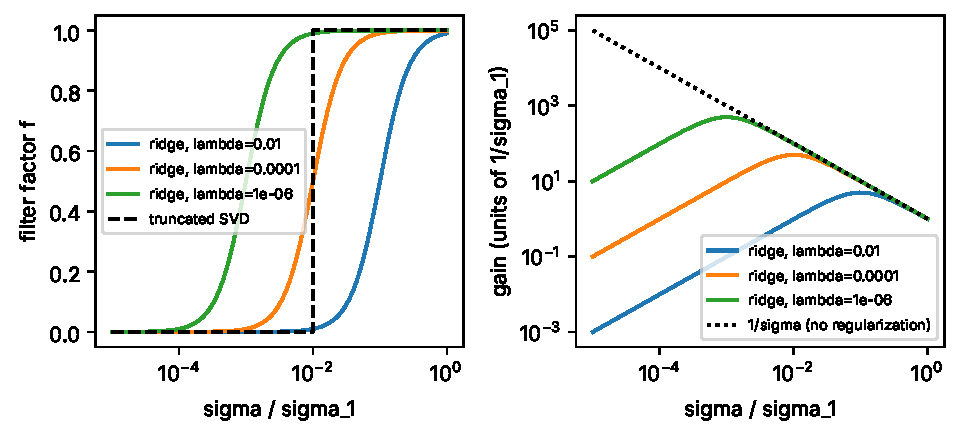
\includegraphics[width=0.95\linewidth]{figs/least-squares_filter.pdf}
\caption{Left: filter factors $f$ against $\sigma/\sigma_1$ for ridge regularization, $f=\sigma^2/(\sigma^2+\lambda\sigma_1^2)$, with $\lambda = 10^{-2}, 10^{-4}, 10^{-6}$ (solid), and for a truncated SVD that keeps $\sigma/\sigma_1\ge10^{-2}$ (dashed step). Right: the gain applied to the data component along $u_j$, in units of $1/\sigma_1$: the unregularized $1/\sigma$ grows without bound, while the ridge gain $\sigma/(\sigma^2+\lambda\sigma_1^2)$ peaks at $\sigma=\sqrt\lambda\,\sigma_1$ with height $1/(2\sqrt\lambda\,\sigma_1)$. All quantities dimensionless.}\label{fig:least-squares-filter}
\end{figure}

\begin{sample}{Ridge versus truncation on a two-coefficient problem}
Take $A = \mathrm{diag}(1,\ 0.01)$ and true coefficients $c_{\rm true} = (1,1)$, so the true data are $(1,\ 0.01)$. The measurement of the second component carries an error of $+0.01$: $y = (1,\ 0.02)$. Compare the plain solution, the truncated SVD with $J = 1$, and ridge with $\alpha = 10^{-5}, 10^{-4}, 10^{-3}$.

\textbf{Step 1: SVD.} $A$ is diagonal with positive entries, so $U = V = I$, $\sigma_1 = 1$, $\sigma_2 = 0.01$, $\kappa = 100$, and $u_j^\top y = y_j$.

\textbf{Step 2: plain solution.} $c^+ = (y_1/\sigma_1,\ y_2/\sigma_2) = (1,\ 2)$. The noise $0.01$ was divided by $\sigma_2 = 0.01$: an error of $1$ in $c_2$. Error norm $\norm{c - c_{\rm true}} = 1$.

\textbf{Step 3: truncated SVD.} Keeping only $j=1$: $c^{(1)} = (1,\ 0)$. The noise is gone, and so is the true value of $c_2$. Error norm $1$.

\textbf{Step 4: ridge.} By \cref{eq:least-squares-ridge-svd}, $c_1 = 1\cdot1/(1+\alpha)$ and $c_2 = 0.01\cdot0.02/(10^{-4}+\alpha) = 2\times10^{-4}/(10^{-4}+\alpha)$:

\begin{center}
\begin{tabular}{cccc}\toprule
$\alpha$ & $c_1$ & $c_2$ & $\norm{c_\alpha - c_{\rm true}}$\\\midrule
$10^{-5}$ & 0.99999 & 1.8182 & 0.818\\
$10^{-4}$ & 0.99990 & 1.0000 & $1.0\times10^{-4}$\\
$10^{-3}$ & 0.99900 & 0.1818 & 0.818\\\bottomrule
\end{tabular}
\end{center}

\textbf{Step 5: interpret.} $c_1$ barely notices the regularization (its $\sigma$ is far above $\sqrt\alpha$). For $c_2$, too little regularization leaves the noise in, too much removes the signal. At $\alpha = 10^{-4}$ the filter factor for $j=2$ is exactly $\frac12$, which here happens to cancel the noise exactly, because in this example the noise ($0.01$) equals the true signal ($0.01$). Such a perfect result is a coincidence of this example; Problem~25 finds the best $\alpha$ when the noise is known only on average.
\[
\boxed{\,\text{plain: }(1,2);\quad \text{TSVD: }(1,0);\quad \text{ridge }\alpha=10^{-4}: (0.9999,\,1.0000)\,}
\]
\end{sample}

\paragraph{Choosing the regularization strength.} The sample shows that the best $\alpha$ depends on the noise, which in practice you do not know. Using the data you are fitting to choose $\alpha$ fails (the in-sample error is smallest at $\alpha=0$). The standard remedy is \emph{validation}: fit with several values of $\alpha$ on part of the data and pick the value that best predicts the rest. Chapters~\ref{ch:generalization} and~\ref{ch:sparse-frequency} develop this; the paper's fitted controls choose their ridge strength by such a forward split (\cref{sec:least-squares-paper}).

\begin{pitfall}
Ridge penalizes $\norm{c}^2$, so ``small'' is measured in your chosen parametrization. Multiply one basis function by 10 and the coefficient needed to produce the same model drops tenfold, which the penalty treats as much cheaper. Ridge (and the minimum-norm solution) therefore depend on how the basis is scaled and which basis is used. Regularization expresses a preference; it does not by itself discover the right model.
\end{pitfall}

\begin{pycode}
import numpy as np

def ridge_svd(A, y, lam):
    """Ridge solution with alpha = lam * sigma_1**2, Eq. (ridge-rel)."""
    U, s, Vh = np.linalg.svd(A, full_matrices=False)
    gain = s / (s**2 + lam * s[0]**2)      # sigma/(sigma^2 + lam sigma_1^2)
    return Vh.T @ (gain * (U.T @ y))

A = np.diag([1.0, 0.01])
y = np.array([1.0, 0.02])
for lam in [1e-5, 1e-4, 1e-3]:
    print(lam, ridge_svd(A, y, lam))       # reproduces the sample's table
\end{pycode}

\begin{checkpoint}
As $\alpha$ is increased from $0$ to very large values, what happens to the in-sample residual $\norm{y - Ac_\alpha}$?
\end{checkpoint}
\checkanswer{It never decreases. At $\alpha = 0$ the residual is as small as any $c$ can make it; as $\alpha\to\infty$, $c_\alpha\to0$ and the residual approaches $\norm{y}$, the residual of doing nothing. Ridge trades in-sample accuracy for smaller coefficients.}

\begin{keyideas}
\item Ridge minimizes $\norm{y-Ac}^2+\alpha\norm{c}^2$; its solution $(A^\top A+\alpha I)^{-1}A^\top y$ always exists and is unique (\cref{eq:least-squares-ridge-normal}).
\item In SVD form the data along $u_j$ are multiplied by $\sigma_j/(\sigma_j^2+\alpha)$ (\cref{eq:least-squares-ridge-svd}); filter factors $\sigma_j^2/(\sigma_j^2+\alpha)$.
\item With $\alpha = \lambda\sigma_1^2$ the filter is $\sigma/(\sigma^2+\lambda\sigma_1^2)$, the paper's form (\cref{eq:least-squares-ridge-rel}).
\item $\alpha\to0$ gives the minimum-norm solution; $\alpha\to\infty$ gives $c=0$ (the null); the gain never exceeds $1/(2\sqrt\alpha)$.
\end{keyideas}

%======================================================================
\section{Overfitting: the memorizing polynomial}\label{sec:least-squares-overfit}

Least squares makes the residuals on the data as small as possible. That is a statement about the data you have. This section shows, with the book's running example RE4, why it is not a statement about the data you do not have.

\paragraph{The data.} We sample $\sin t$ at ten equally spaced times $t_j = 0.7j$, $j = 0,\dots,9$, and add fixed ``measurement errors'' $\varepsilon_j$ of size $0.10$ to $0.15$ (\cref{tab:least-squares-re4}). We chose the errors to alternate in sign, which makes the effect below easy to see; Problem~18 asks you to repeat the experiment with random errors.

\begin{table}[htbp]\centering
\caption{The RE4 data: $y_j = \sin t_j + \varepsilon_j$ at $t_j = 0.7j$.}\label{tab:least-squares-re4}
\small
\begin{tabular}{ccccccccccc}\toprule
$j$ & 0 & 1 & 2 & 3 & 4 & 5 & 6 & 7 & 8 & 9\\\midrule
$t_j$ & 0 & 0.7 & 1.4 & 2.1 & 2.8 & 3.5 & 4.2 & 4.9 & 5.6 & 6.3\\
$\sin t_j$ & 0.0000 & 0.6442 & 0.9854 & 0.8632 & 0.3350 & $-0.3508$ & $-0.8716$ & $-0.9825$ & $-0.6313$ & 0.0168\\
$\varepsilon_j$ & 0.15 & $-0.12$ & 0.10 & $-0.15$ & 0.12 & $-0.10$ & 0.14 & $-0.13$ & 0.11 & $-0.14$\\
$y_j$ & 0.1500 & 0.5242 & 1.0855 & 0.7132 & 0.4550 & $-0.4508$ & $-0.7316$ & $-1.1125$ & $-0.5213$ & $-0.1232$\\\bottomrule
\end{tabular}
\end{table}

\paragraph{Polynomial models and their conditioning.} We fit polynomials of degree $d$, which have $M = d+1$ coefficients. Rather than powers of $t$ we use powers of the rescaled variable $\tau = t/3.15 - 1$, which runs from $-1$ to $1$ over the data. (We write $\tau$ rather than $u$ because $u_j$ already denotes the left singular vectors.) A polynomial of degree $d$ in $\tau$ is a polynomial of degree $d$ in $t$ and vice versa, so this changes only the coordinates in coefficient space, not the set of models or the fitted curve. It does change the conditioning. With powers of $t$, the column $t^9$ has entries up to $6.3^9\approx1.6\times10^7$ while the column $1$ has length $\sqrt{10}$, and Problem~27 shows this forces $\kappa > 10^6$; in the variable $\tau$ the condition number is far smaller: the listing below prints both condition numbers, and the first exceeds the second by more than a factor 100. Choosing a well-scaled basis is the first line of defense of \cref{sec:least-squares-cond}.

\begin{pycode}
import numpy as np
t = 0.7 * np.arange(10)          # the RE4 times
tau = t / 3.15 - 1                 # rescaled to [-1, 1]
print(np.linalg.cond(np.vander(t, 10)))   # columns t^9, ..., t, 1
print(np.linalg.cond(np.vander(tau, 10)))   # columns tau^9, ..., tau, 1
\end{pycode}

\paragraph{Three fits.} \Cref{fig:least-squares-poly} shows the least-squares polynomials of degree $1$, $3$ and $9$.
\begin{itemize}
\item Degree 1 (a line) is too stiff to follow one full oscillation of $\sin t$: it \emph{underfits}.
\item Degree 3 follows the overall shape and smooths through the errors.
\item Degree 9 has $M=10$ coefficients for $m = 10$ points. The design matrix is square, and it is invertible because the times are distinct: if $Ac = 0$, the polynomial with coefficients $c$ vanishes at ten distinct points, but a nonzero polynomial of degree at most $9$ has at most $9$ roots, so $c = 0$. (The root count follows from the factor theorem of school algebra: if $t_0$ is a root, the polynomial equals $(t-t_0)$ times a polynomial of one lower degree, so each distinct root uses up one degree.) Hence the degree-9 polynomial passes \emph{exactly} through every data point, errors included. To do so it must wiggle, and between the data points, especially near the ends of the range, it swings far from $\sin t$.
\end{itemize}

\begin{figure}[htbp]\centering
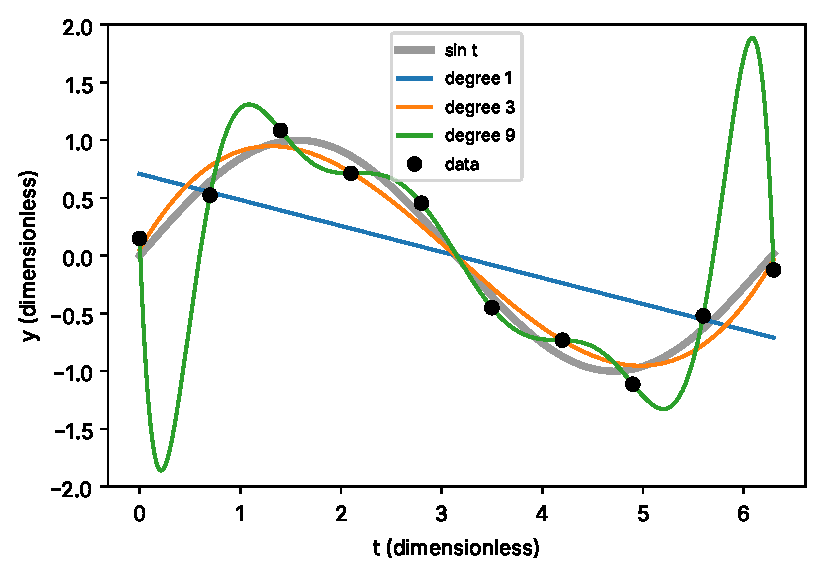
\includegraphics[width=0.85\linewidth]{figs/least-squares_poly.pdf}
\caption{The memorizing polynomial (RE4). Points: the ten noisy samples of \cref{tab:least-squares-re4}. Gray: $\sin t$. Least-squares polynomials of degree 1 (underfits), 3 (follows the shape) and 9 (passes through every point, errors included, and oscillates between them). Horizontal axis: $t$ (dimensionless); vertical axis: $y$ (dimensionless).}\label{fig:least-squares-poly}
\end{figure}

\paragraph{Training error versus test error.} The root mean square (rms) of numbers $r_1,\dots,r_m$ is $\sqrt{\frac1m\sum_i r_i^2} = \norm{r}/\sqrt m$. Call the rms residual on the ten data points the \emph{training error}, and the rms difference between the fitted polynomial and $\sin t$ over the whole interval $0\le t\le6.3$ the \emph{test error} (it measures how well the fit predicts values it was not given). \Cref{fig:least-squares-degree} plots both against degree.

The training error can never increase with degree. Proof: every polynomial of degree $d-1$ is also a polynomial of degree $d$ (with top coefficient zero), so the minimum of $S$ over degree-$d$ models is taken over a larger set and can only be smaller or equal. At $d = 9$ it reaches zero (up to rounding). The test error behaves differently: it falls from degree 1 to degree 3, and at degree 9 it is more than twice as large as at degree 3. Driving the training error to zero did not make the predictions better; it made them worse, because the extra coefficients were spent fitting the errors $\varepsilon_j$. This is \emph{overfitting}, and a model that reproduces its training data exactly, errors included, has \emph{memorized} them.

\begin{figure}[htbp]\centering
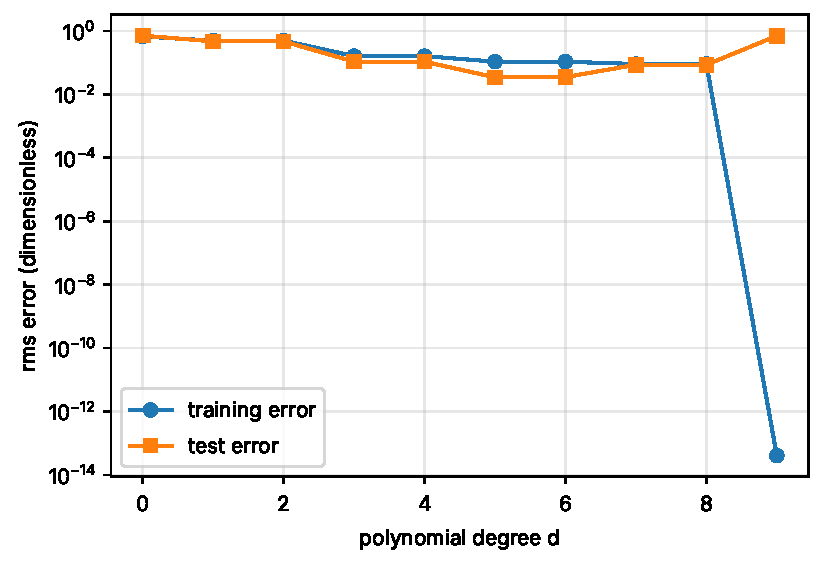
\includegraphics[width=0.85\linewidth]{figs/least-squares_degree.pdf}
\caption{Training error (rms residual on the ten RE4 points) and test error (rms deviation from $\sin t$ on $0\le t\le 6.3$) of least-squares polynomials against degree $d$. The training error never increases and reaches zero, to rounding, at $d=9$ (plotted at a floor of $10^{-16}$); the test error at $d=9$ is more than twice that at $d=3$. Errors dimensionless, log scale.}\label{fig:least-squares-degree}
\end{figure}

If we go further, to degree $15$ (16 coefficients, 10 data), the problem is underdetermined: by \cref{sec:least-squares-pinv} there is a null space of dimension at least $6$ and infinitely many polynomials that pass exactly through all ten points. \texttt{lstsq} returns the minimum-norm one. They all have training error zero, so the training data cannot tell them apart at all, yet between and beyond the points they differ arbitrarily (add any null vector). Ridge regularization of the degree-9 or degree-15 fit pulls the coefficients toward zero, at the cost of a nonzero training error; whether that improves the predictions is examined, with the tools of statistics, in Chapter~\ref{ch:generalization}.

\begin{sample}{Interpolation versus extrapolation with three points}
Three points of $\sin t$ are known exactly: $(0,0)$, $(\pi/2,1)$, $(\pi,0)$. Fit (a) a least-squares line and (b) the parabola through all three, and use each to predict $\sin t$ at $t=\pi/4$ (inside the data range) and at $t = 3\pi/2$ (outside it).

\textbf{Step 1: line sums.} $m = 3$; $\sum t_i = 3\pi/2$; $\sum t_i^2 = 0 + \pi^2/4 + \pi^2 = 5\pi^2/4$; $\sum y_i = 1$; $\sum t_iy_i = \pi/2$.

\textbf{Step 2: line normal equations.} $3c_0 + \frac{3\pi}{2}c_1 = 1$ and $\frac{3\pi}{2}c_0 + \frac{5\pi^2}{4}c_1 = \frac\pi2$. Multiply the first by $\pi/2$: $\frac{3\pi}{2}c_0 + \frac{3\pi^2}{4}c_1 = \frac\pi2$. Subtract from the second: $\frac{\pi^2}{2}c_1 = 0$, so $c_1 = 0$ and $c_0 = \frac13$. The line is $y = \frac13$.

\textbf{Step 3: parabola.} Write $y = c_0 + c_1t + c_2t^2$. Through $(0,0)$: $c_0 = 0$. Through $(\pi,0)$: $c_1\pi + c_2\pi^2 = 0$, so $c_1 = -c_2\pi$. Through $(\pi/2,1)$: $c_1\frac\pi2 + c_2\frac{\pi^2}{4} = 1$, i.e.\ $-c_2\frac{\pi^2}{2}+c_2\frac{\pi^2}{4} = 1$, so $c_2 = -4/\pi^2$ and $c_1 = 4/\pi$. Hence $y = \frac{4}{\pi^2}\,t(\pi - t)$.

\textbf{Step 4: predictions at $t = \pi/4$} (truth $\sin\frac\pi4\approx0.7071$). Line: $0.3333$, error $0.374$. Parabola: $\frac{4}{\pi^2}\cdot\frac\pi4\cdot\frac{3\pi}{4} = \frac34 = 0.75$, error $0.043$.

\textbf{Step 5: predictions at $t = 3\pi/2$} (truth $-1$). Line: $0.3333$, error $1.333$. Parabola: $\frac{4}{\pi^2}\cdot\frac{3\pi}{2}\cdot\bigl(-\frac\pi2\bigr) = -3$, error $2.0$.
\[
\boxed{\,\text{at }\tfrac\pi4:\ \text{line }0.333,\ \text{parabola }0.75;\qquad \text{at }\tfrac{3\pi}2:\ \text{line }0.333,\ \text{parabola }-3\,}
\]
Inside the data range the flexible exact fit wins easily; outside it, both models fail and the exact fit fails worse. Neither ``knows'' that the function oscillates. Predicting outside the range of the data, \emph{extrapolation}, needs a model whose form matches the truth.
\end{sample}

\paragraph{The right basis.} What happens if the basis does contain the true form? The next sample uses the book's running example RE2, the prime-2 wave of Chapter~\ref{ch:fourier-series},
\begin{equation}
F_2(t) = -\frac1\pi\sum_{m=1}^{3}\frac{\sin(mt\log2)}{m\,2^{m/2}} ,
\label{eq:least-squares-re2}
\end{equation}
which repeats with period $2\pi/\log 2\approx 9.065$ in $t$. (Here $m$ is the harmonic index, as in the paper's Eq.~(4), not the number of data points.)

\begin{sample}{Least squares recovers the prime-2 wave}
Sample $F_2$ of \cref{eq:least-squares-re2} at the first ten zeta-zero heights of RE1 ($t = 14.134725,\dots,49.773832$) and fit the six-coefficient model $\sum_{m=1}^3\bigl[a_m\sin(mt\log2) + b_m\cos(mt\log 2)\bigr]$ by least squares. What coefficients come out, and how well does the fit predict $F_2$ at other $t$?

\textbf{Step 1: design matrix.} Ten rows (one per $t_i$), six columns: $\sin(t_i\log2)$, $\cos(t_i\log2)$, $\sin(2t_i\log2)$, $\cos(2t_i\log 2)$, $\sin(3t_i\log 2)$, $\cos(3t_i\log2)$. Applying \texttt{numpy.linalg.matrix\_rank} to this matrix (the listing after this sample) returns $6$: its columns are independent, so the least-squares solution is unique.

\textbf{Step 2: the true coefficients fit exactly.} The data are $F_2(t_i)$, which is itself of the model form with $a_m = -1/(\pi m2^{m/2})$ and $b_m = 0$. With these coefficients every residual is zero, so $S = 0$, the smallest possible value. A minimizer of $S$ is therefore this coefficient vector, and by uniqueness it is the only one.

\textbf{Step 3: values.} $a_1 = -1/(\pi\sqrt2)\approx -0.22508$, $a_2 = -1/(4\pi)\approx-0.07958$, $a_3 = -1/(6\sqrt2\,\pi)\approx -0.03751$, $b_1 = b_2 = b_3 = 0$. A numerical \texttt{lstsq} reproduces these to rounding error.

\textbf{Step 4: prediction.} With the exact coefficients the model \emph{is} $F_2$, so it predicts $F_2$ at every $t$, far outside the sampled window included.
\[
\boxed{\,a = (-0.22508,\,-0.07958,\,-0.03751),\quad b = 0;\ \text{prediction exact for all } t\,}
\]
\end{sample}

\begin{pycode}
import numpy as np
t = np.array([14.134725, 21.022040, 25.010858, 30.424876, 32.935062,
              37.586178, 40.918719, 43.327073, 48.005151, 49.773832])
w = np.log(2) * np.array([1, 2, 3])
D = np.hstack([np.sin(np.outer(t, w)), np.cos(np.outer(t, w))])
print(np.linalg.matrix_rank(D))               # 6
F = -sum(np.sin(m*t*np.log(2))/(m*2**(m/2)) for m in (1, 2, 3))/np.pi
print(np.linalg.lstsq(D, F, rcond=None)[0])   # a1, a2, a3, then b's near 0
\end{pycode}

Contrast this with a generic basis. \Cref{fig:least-squares-re2} fits the same wave, sampled at 80 equally spaced points in $10\le t\le60$, with $120$ sinusoids whose frequencies lie on a uniform grid that does not contain $\log2$, $2\log 2$ or $3\log2$. With 120 coefficients and 80 data the problem is underdetermined, and the minimum-norm solution fits the samples in the window essentially exactly. Beyond the window it drifts away from the true wave, while the three-frequency model continues it perfectly. The moral, developed in Chapters~\ref{ch:generalization} and~\ref{ch:sparse-frequency}: \emph{a fit generalizes when its basis encodes the right structure, not when it has many coefficients}.

\begin{figure}[htbp]\centering
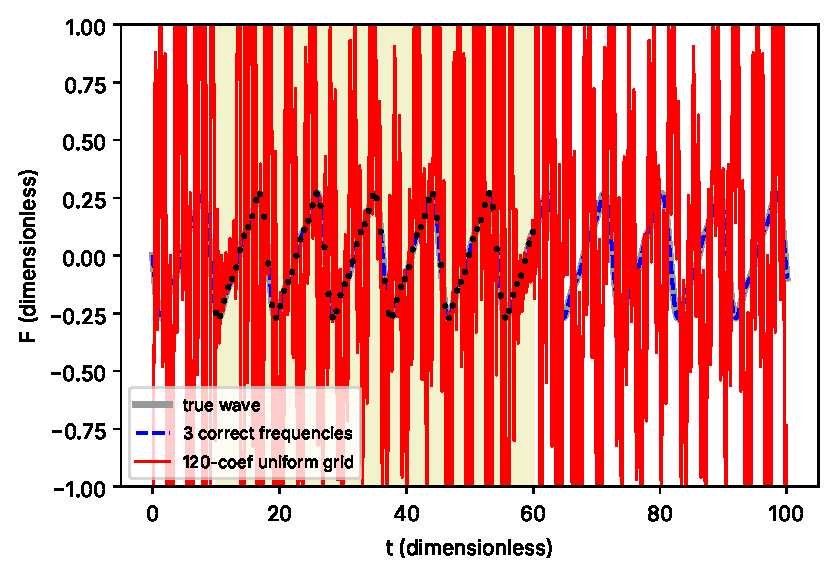
\includegraphics[width=0.85\linewidth]{figs/least-squares_re2.pdf}
\caption{Fitting the prime-2 wave RE2 (\cref{eq:least-squares-re2}) from 80 samples in the shaded window $10\le t\le60$. Gray: the true wave. Dashed: least-squares fit with the three correct frequencies $m\log2$ (6 coefficients), which continues the wave exactly. Solid: minimum-norm fit with 120 coefficients on a uniform frequency grid $\omega_j = 8j/60$, $j=1,\dots,60$, which matches the samples in the window but drifts away from the wave outside it. $t$ and $F$ dimensionless.}\label{fig:least-squares-re2}
\end{figure}

\begin{checkpoint}
A friend fits 50 data points with a 60-coefficient model and reports ``zero residual on all 50 points, so the model is correct.'' What is wrong with the argument?
\end{checkpoint}
\checkanswer{With more coefficients than data, an exact fit is expected for almost any data (\cref{sec:least-squares-pinv}), and there are infinitely many exact fits differing by null-space vectors. Zero training residual says nothing about predictions at new points; only a test on held-out data can.}

\begin{keyideas}
\item Training error never increases as you add basis functions; with as many coefficients as data it is zero.
\item A model that fits its training data exactly, errors included, has memorized them; its predictions elsewhere can be poor (RE4).
\item In these examples extrapolation succeeded when the model family contained the true form (RE2 with the right frequencies) and failed for a large generic basis, which fits the window but not beyond it; more coefficients did not help.
\end{keyideas}

%======================================================================
\section{Paper connection}\label{sec:least-squares-paper}

This section reads the least-squares content of the paper \cite{soniR1} line by line. Quantities such as energy levels $E_n$ and wavefunctions $\psi_n$ are explained in Part~II (Chapters~\ref{ch:schrodinger} and~\ref{ch:perturbation}) and in Chapter~\ref{ch:finite-differences}; here we need only that they are numbers and vectors computed from a matrix.

\paragraph{The fit is a sequence of least-squares problems (Sec.~II~C).} The paper adds to the Wu--Sprung potential a correction $\delta V(x) = \sum_{k=0}^{M-1}c_k\cos(k\pi x/L)$, a linear model in the coefficients $c_k$ with the cosine basis of Chapter~\ref{ch:fourier-series}. The energy levels $E_n$ depend on $c$ nonlinearly, so the fit proceeds by ``iterated linearization'': compute the levels $E_n$ and wavefunctions $\psi_n$ for the current $c$, form residuals $r_n = \tilde t_n - E_n$ (target minus model, exactly as in \cref{eq:least-squares-resid}; $\tilde t_n$ are the bias-corrected zero heights of Chapter~\ref{ch:finite-differences}), and form the first-order sensitivity matrix
\[
A_{nk} = \int\abs{\psi_n}^2\cos(k\pi x/L)\,\dd x .
\]

\begin{beyond}
\textbf{Taken on trust until Chapter~\ref{ch:perturbation}.} The energy levels $E_n$ and normalized wavefunctions $\psi_n$ are defined in Chapters~\ref{ch:schrodinger} and~\ref{ch:bound-states}; here treat them as numbers and functions computed from the current potential. First-order perturbation theory, derived in Chapter~\ref{ch:perturbation}, states that a small change $\delta c$ of the coefficients changes level $n$ by approximately $\sum_k A_{nk}\delta c_k$, with an error of second order in $\delta c$. We use this fact here without proof.
\end{beyond}

To first order, then, choosing the change $\delta c$ that best removes the residuals is the linear least-squares problem
\begin{equation}
A\,\delta c\approx r ,
\label{eq:least-squares-paper-lin}
\end{equation}
with $A$ playing the role of the design matrix (rows: training levels $n$; columns: basis functions $k$) and $r$ the role of the data. (Do not confuse this matrix $A_{nk}$ with the non-Hermitian operator $A$ of the paper's Sec.~II~E; the paper uses the letter for both.)

\paragraph{Decoding Appendix~A step~6.} The paper's record states the update as
\[
c \mathrel{+}= V\!\left(\Sigma/(\Sigma^2+\lambda\Sigma_1^2)\right)U^\top r ,
\]
with a ``try-list $(0.2\lambda,\lambda,5\lambda,25\lambda)$''. In the notation of this chapter, $A = U\Sigma V^\top$ is the SVD of the sensitivity matrix, $\Sigma$ the diagonal of singular values and $\Sigma_1 = \sigma_1$ the largest one, and the division is entry by entry. Here $V$ is the matrix of right singular vectors, \emph{not} the potential $V(x)$: another overloaded letter. Comparing with \cref{eq:least-squares-ridge-rel}, the step is
\begin{equation}
\delta c = \sum_j\frac{\sigma_j}{\sigma_j^2+\lambda\sigma_1^2}\,(u_j^\top r)\,v_j ,
\label{eq:least-squares-paperstep}
\end{equation}
which is precisely the ridge solution of \cref{eq:least-squares-paper-lin}: the $\delta c$ that minimizes $\norm{r - A\delta c}^2 + \lambda\sigma_1^2\norm{\delta c}^2$. Damping the \emph{step} in this way is the Levenberg--Marquardt idea \cite{marquardt}, developed in Chapter~\ref{ch:fitting}. In this step $\lambda$ is the Levenberg--Marquardt damping (the book's notation, Appendix~B: $\lambda$ for damping, $\mu$ for ridge strength). Two limits make its role concrete (Problem~17):
\begin{itemize}
\item $\lambda\to0$: $\delta c\to A^+r$, the full minimum-norm linearized step (Gauss--Newton);
\item large $\lambda$: $\sigma_j/(\sigma_j^2+\lambda\sigma_1^2)\approx\sigma_j/(\lambda\sigma_1^2)$, so $\delta c\approx V\Sigma^\top U^\top r/(\lambda\sigma_1^2) = A^\top r/(\lambda\sigma_1^2)$, a short step along $A^\top r$. The \emph{gradient} of $S$ is the vector of its partial derivatives, $(\partial S/\partial c_1,\dots,\partial S/\partial c_M) = -2A^\top r$ by \cref{eq:least-squares-grad}, so $A^\top r$ points opposite to the gradient. A small step in this direction decreases $S$ fastest (shown in Chapter~\ref{ch:fitting}), which is why it is called the direction of \emph{steepest descent}.
\end{itemize}
Because each component of \cref{eq:least-squares-paperstep} shrinks as $\lambda$ grows, larger $\lambda$ always means a shorter, more cautious step. According to the record, a step is accepted only if it lowers the rms by the factor $0.999$ (``accept only improvements ($\times0.999$)''; one row of Table~I, scale~2 with $M=300$, used the looser threshold $1-10^{-5}$, and the paper reports that row as a sensitivity result); on success $\lambda\leftarrow\max(0.5\lambda_{\rm acc},10^{-7})$, on failure of every value in the try-list $\lambda\leftarrow30\lambda$, and the iteration stops when $\lambda>10^4$. Chapter~\ref{ch:fitting} explains this schedule; the linear algebra inside each step is this chapter's.

\begin{sample}{One damped step in miniature}
Apply the step \cref{eq:least-squares-paperstep} with $\lambda = 0.01$ to the matrix $A = \begin{pmatrix}3&0\\4&5\end{pmatrix}$ of the earlier SVD sample and residual $r = (1,1)$, and compare with the undamped step $A^{-1}r$.

\textbf{Step 1: SVD (from the earlier sample).} $\sigma_1 = 3\sqrt5$, $\sigma_2 = \sqrt5$, $u_1 = (1,3)/\sqrt{10}$, $u_2 = (3,-1)/\sqrt{10}$, $v_1 = (1,1)/\sqrt2$, $v_2 = (1,-1)/\sqrt2$.

\textbf{Step 2: data components.} $u_1^\top r = 4/\sqrt{10}\approx1.26491$; $u_2^\top r = 2/\sqrt{10}\approx0.63246$.

\textbf{Step 3: damped gains.} $\lambda\sigma_1^2 = 0.01\times45 = 0.45$. Gain 1: $\sigma_1/(\sigma_1^2+0.45) = 6.70820/45.45\approx0.147595$. Gain 2: $\sigma_2/(\sigma_2^2+0.45) = 2.23607/5.45\approx0.410288$.

\textbf{Step 4: assemble.} $\delta c = 0.147595\times1.26491\,v_1 + 0.410288\times0.63246\,v_2 = 0.186695\,v_1 + 0.259489\,v_2$. With $v_{1,2} = (1,\pm1)/\sqrt2$: $\delta c = \bigl((0.186695+0.259489)/\sqrt2,\ (0.186695-0.259489)/\sqrt2\bigr)\approx(0.3155,\ -0.0515)$.

\textbf{Step 5: undamped step.} Solving $A\delta c = r$: $3\delta c_1 = 1$ gives $\delta c_1 = 1/3$; then $4/3 + 5\delta c_2 = 1$ gives $\delta c_2 = -1/15\approx-0.0667$.
\[
\boxed{\,\delta c_{\lambda=0.01}\approx(0.3155,\,-0.0515)\quad\text{vs}\quad A^{-1}r = (0.3333,\,-0.0667)\,}
\]
The damped step is shorter; the component along the weaker direction $v_2$ is shrunk more (gain $0.410$ instead of $1/\sigma_2 = 0.447$) than the one along $v_1$ (gain $0.1476$ instead of $1/\sigma_1 = 0.1491$).
\end{sample}

\paragraph{What the sensitivity matrix looks like.} \Cref{fig:least-squares-sensitivity} shows the singular values of $A_{nk}$ computed with the companion library \texttt{qmnt} for the unperturbed potential (the first iteration of the fit, $c=0$) in the scale-1 box of RE3 ($L = 44.883$, the paper's working grid $N=6000$), for the first 400 levels and $M = 400$ or $900$ cosines. One column is known exactly: for $k=0$, $\cos0 = 1$ and $A_{n0} = \int\abs{\psi_n}^2\dd x = 1$ for every level, because the wavefunctions are normalized. A constant shift of the potential raises every level by the same amount. A $400\times900$ matrix has at most 400 nonzero singular values, so at $M = 900$ at least 500 directions of coefficient space are invisible to the 400 training levels, to first order. Read the figure with \cref{sec:least-squares-cond} in mind. Directions $v_j$ whose normalized singular value $\sigma_j/\sigma_1$ lies far below 1 are poorly constrained by the training levels, and the damping filter of \cref{eq:least-squares-paperstep} shrinks the step along them much more than along the well-constrained directions.

\begin{figure}[htbp]\centering
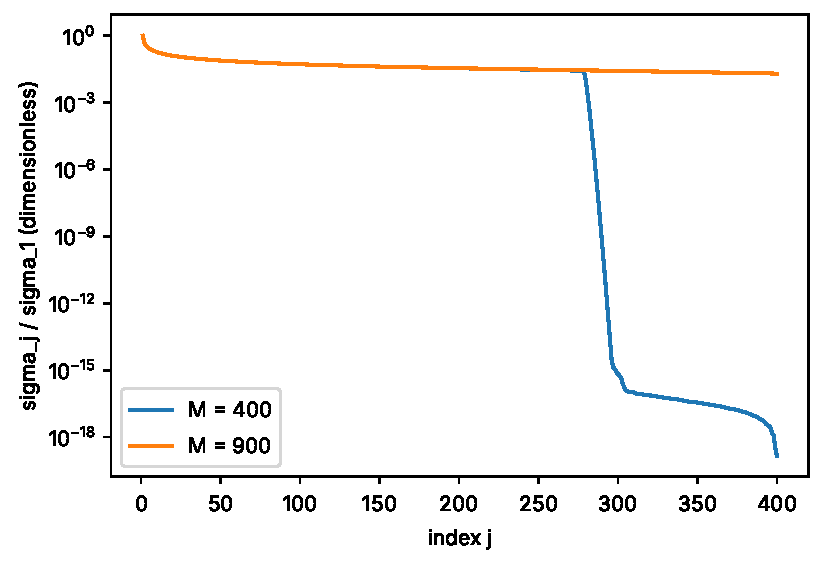
\includegraphics[width=0.85\linewidth]{figs/least-squares_sensitivity.pdf}
\caption{Normalized singular values $\sigma_j/\sigma_1$ of the first-order sensitivity matrix $A_{nk}=\int\abs{\psi_n}^2\cos(k\pi x/L)\,\dd x$ of the paper's Sec.~II~C, for the first 400 levels of the unperturbed Wu--Sprung potential in the scale-1 box ($L=44.883$, $N=6000$ interior grid points, units $\hbar=2m=1$), with $M=400$ and $M=900$ cosine basis functions. The $400\times900$ matrix has only 400 singular values; the remaining 500 directions of its coefficient space form (at least) its null space. Computed with \texttt{qmnt}.}\label{fig:least-squares-sensitivity}
\end{figure}

\paragraph{Ridge in the operator fits (Tables~I and~II, Sec.~III).} The record says the ``ridge variant adds $\mu\Sigma_1^2$ to the filter denominator''. In the language of \cref{sec:least-squares-ridge}, $\mu$ is a ridge strength measured relative to $\sigma_1^2$, entering the same filter denominator as $\lambda$ in \cref{eq:least-squares-ridge-rel}, but playing a different role. The damping $\lambda$ is adapted during the iteration and driven small after successful steps, so it controls only how long each step is: iterated to convergence, a damped step need not change where the fit ends up. The ridge term $\mu\sigma_1^2$ is fixed and stays in the filter at every step, so the steps never become full Gauss--Newton steps along poorly constrained directions. This chapter does not derive how a fixed $\mu$ in the step filter changes the converged fit. The full specification of how the ridge enters the iteration is in the paper's Zenodo record \cite{zenodo}, and Chapter~\ref{ch:fitting} discusses it. The effect matches the limits derived in \cref{sec:least-squares-ridge}. In Table~I (scale 1, fit zeros 1--400, $M=400$), the unregularized fit has in-sample rms $0.137$ and held-out rms $0.369$; with $\mu = 0.03$ these become $0.142$ and $0.271$; with $\mu = 0.3$, $0.206$ and $0.265$, against a null of $0.263$ on zeros 401--500 (RE5). As ridge strength grows, the in-sample error rises (the fit memorizes less) and the held-out error approaches the null from above: the fitted correction stays closer to $c = 0$, ``doing nothing''. The paper summarizes: ``regularization moves them smoothly from `memorize more' to `do nothing' and never creates skill'' (Sec.~III). Table~II shows the same for the Chebyshev basis ($\mu = 0.3$: held-out $0.264$), and in the interpolation split of Sec.~III ridge brings the gap error from $2.64$ spacings back to $0.262$ ($\mu=0.03$) and $0.257$ ($\mu=0.3$), close to that split's null $0.255$. This behavior is consistent with the picture of \cref{sec:least-squares-cond}: ridge suppresses large excursions along poorly constrained directions (\cref{eq:least-squares-noise}), and it cannot add information the parametrization lacks. The paper's own explanation of the gap damage is heuristic and stated in its own terms: the optimizer ``places large structure in the part of the potential that only the held-out levels probe strongly, because doing so costs nothing in-sample'' (Sec.~III). The paper does not attribute the damage to noise amplification, and neither do we.

\paragraph{Saturated fits (Sec.~III, Table~III).} Sec.~III reports that on all 500 scale-1 zeros the fit reaches rms $0.186$ at $M = 300$ and reproduces all 500 to rms $<10^{-4}$ spacings by $M = 900$. With 900 coefficients and 500 levels, the linearized problem \cref{eq:least-squares-paper-lin} is underdetermined: if the $500\times900$ matrix has full row rank, exact fits exist and differ by vectors of a null space of dimension at least $400$ (\cref{sec:least-squares-pinv}). The underlying problem is nonlinear, so this is a first-order heuristic, but it suggests why near-perfect in-sample agreement is unsurprising and, by analogy with RE4, why such agreement need not carry information about held-out levels. (This argument is ours; the paper reports the observation, not this derivation.) Similarly, Sec.~III notes that the odd/even splits of Table~III have 200 training levels at scale~1, ``so the rows with $M \ge 200$ are saturated''; at $M = 400$ the in-sample error is below $10^{-3}$.

\paragraph{The fitted sinusoidal controls (Secs.~II~D and~IV, Table~IV, Appendix~A step~20).} The controls fit $F(t) = \sum_j[a_j\sin(\omega_jt)+b_j\cos(\omega_jt)]$ to $y_n = n-\tfrac12 - \Nsm(t_n)$ at the training zeros ``by least squares''. (Here $\Nsm$ is the smooth zero-counting function of the paper's Eq.~(1), Chapter~\ref{ch:counting-zeros}; for the least squares it is just a known function of $t$.) With fixed frequencies this is linear least squares exactly as in the RE2 sample, with $2$ coefficients per frequency. Control B supplies the frequencies $m\log p$ ($m\le3$): with 25 primes that is $25\times3\times2 = 150$ coefficients, which ``learned from 400 zeros give $0.028$''. With 150 primes it is $900$ coefficients, and the paper writes: ``At 900 coefficients on 400 zeros the least-squares problem is underdetermined and the model degrades to $0.180$ with correlation $+0.78$'' (Sec.~IV); \cref{sec:least-squares-pinv} explains the word: 400 equations, 900 unknowns, a null space of dimension at least 500, regularized only by the ridge. With 800 training zeros it gives $0.100/{+0.94}$ (Table~IV); note that even then $900 > 800$, so the problem is still underdetermined, with a null space of dimension at least 100 (Problem~15). Control C1 uses $450$ frequencies on the uniform grid $\omega_j = 8j/450$, again $900$ coefficients, and stays within $0.005$ of the null ($0.258$ against $0.263$): the generic-basis lesson of \cref{fig:least-squares-re2} at full scale.

Appendix~A step~20 gives the controls' ``ridge filter $\Sigma/(\Sigma^2+\lambda\Sigma_1^2)$, $\lambda = 10^{-8},\dots,10^3$ in half decades'', which is \cref{eq:least-squares-ridge-rel} with $\lambda$ now a ridge strength (in step~6 the same letter is the damping). ``In half decades'' means exponents $-8, -7.5,\dots,3$: $23$ candidate values. The value is chosen by a forward split inside the training window (``first 75\% fit, last 25\% validate'', Sec.~II~D), the validation idea of \cref{sec:least-squares-ridge}; held-out zeros are not used. Table~IV's B row at 900 coefficients is also marked root-ambiguous; that issue concerns the level equation, not the least squares, and is treated in Chapter~\ref{ch:sparse-frequency}.

\paragraph{The lesson in one sentence.} Least squares guarantees the best fit to the data it is given, and the SVD tells you which directions of the model those data constrain. Everything the paper measures beyond that, whether a fit predicts held-out zeros, lies outside what least squares can promise, which is why the paper's central test is out of sample (Chapter~\ref{ch:generalization}).

%======================================================================
\section{Summary}\label{sec:least-squares-summary}

\begin{itemize}
\item Least squares minimizes $S(c) = \norm{y - Ac}^2$, the sum of squared residuals of a linear model $\sum_k c_k\phi_k$ with design matrix $A_{ik}=\phi_k(t_i)$ (\cref{eq:least-squares-design,eq:least-squares-S}).
\item Minimizers satisfy the normal equations $A^\top Ac = A^\top y$ (\cref{eq:least-squares-normal}); every solution is a global minimum by \cref{eq:least-squares-min-identity}; it is unique iff the columns of $A$ are independent. For a line, \cref{eq:least-squares-line-sol}.
\item Geometrically, $A\hat c$ is the orthogonal projection of $y$ onto the column space; $\norm{y}^2 = \norm{\hat y}^2+\norm{\hat r}^2$ (\cref{eq:least-squares-pythagoras}).
\item Every matrix has an SVD $A = U\Sigma V^\top = \sum_j\sigma_ju_jv_j^\top$ (\cref{eq:least-squares-svd,eq:least-squares-outer}), with $\sigma_j^2$ the eigenvalues of $A^\top A$.
\item The minimum-norm least-squares solution is $c^+ = A^+y = \sum_j(u_j^\top y/\sigma_j)v_j$ (\cref{eq:least-squares-pinv-sol}); underdetermined problems have infinitely many exact fits $c^++z$, $Az=0$ (\cref{eq:least-squares-general-sol}).
\item The condition number $\kappa=\sigma_1/\sigma_M$ bounds error amplification (\cref{eq:least-squares-cond-bound}); noise along $u_j$ is divided by $\sigma_j$ (\cref{eq:least-squares-noise}); $\kappa(A^\top A) = \kappa^2$ (\cref{eq:least-squares-kappa2}).
\item Truncated SVD and ridge are filters (\cref{eq:least-squares-filter-form}). Ridge solves $(A^\top A+\alpha I)c = A^\top y$ (\cref{eq:least-squares-ridge-normal}), multiplies the data along $u_j$ by $\sigma_j/(\sigma_j^2+\alpha)$ (\cref{eq:least-squares-ridge-svd}), and with $\alpha=\lambda\sigma_1^2$ takes the paper's form (\cref{eq:least-squares-ridge-rel}); its gain never exceeds $1/(2\sqrt\alpha)$ (\cref{eq:least-squares-gain-cap}).
\item Training error never increases with more basis functions; an exact fit of noisy data is memorization (RE4); in the RE2 example, extrapolation worked with the right frequencies and failed with a large generic basis.
\item The paper's fit step (App.~A step~6) is the ridge-damped linearized step (\cref{eq:least-squares-paperstep}); its ridge rows return toward the null; its controls B and C1 are linear least squares, underdetermined at 900 coefficients on 400 zeros.
\end{itemize}

%======================================================================
\section{Problems}\label{sec:least-squares-problems}

\begin{problemlist}
\prob{1}{Find the least-squares line $y = c_0 + c_1t$ through $(0,0)$, $(1,1)$, $(2,3)$. Give the residuals and $S_{\min}$.}

\prob{1}{Show that for any least-squares line with an intercept, the residuals sum to zero. Does this remain true for the proportional model $y = c_1t$ (no intercept)?}

\prob{1}{For the design matrix $A = \begin{pmatrix}1&0\\1&1\\1&2\end{pmatrix}$ compute $A^\top A$, and for $y = (0,1,3)$ compute $A^\top y$. Compare with Problem~1.}

\prob{1}{Find the singular values and condition number of $A = \mathrm{diag}(-4,\,2)$. Where does the minus sign go in the SVD?}

\prob{1}{Find the minimum-norm solution of $3c_1 + 4c_2 = 10$ using the SVD, and its length.}

\prob{1}{Project $y = (1,2,3)$ onto the line spanned by $a = (1,1,1)$. Show that fitting a constant model $y\approx c$ by least squares gives the average of the data.}

\prob{2}{Derive the least-squares slope of the proportional model $y = kt$, and evaluate it for the data of Problem~1.}

\prob{2}{For $A$ with independent columns and $P = A(A^\top A)^{-1}A^\top$, prove that $P^\top = P$, $P^2 = P$, and $(I - P)A = 0$. Interpret $(I-P)y$.}

\prob{2}{Find the SVD of $A = \begin{pmatrix}1&1\\0&0\end{pmatrix}$, its pseudo-inverse, the minimum-norm least-squares solution for $y = (2,3)$, and the residual.}

\prob{2}{Repeat the ridge sample problem with $y = (1,\ 0.015)$. Which $\alpha$ makes the ridge estimate of $c_2$ exactly equal to the true value $1$?}

\prob{2}{A least-squares problem has $\sigma_1 = 10$ and is solved by ridge in the relative form with $\lambda = 10^{-4}$. What is the largest gain any data component can receive, and at which singular value?}

\prob{2}{Compute the condition number of $\begin{pmatrix}1&2\\2&4.001\end{pmatrix}$. Solve $Ac = (3,\ 6.001)$, then change the right-hand side to $(3,\ 6.002)$ and solve again.}

\prob{2}{RE1 meets least squares. Fit a line $t_n\approx c_0 + c_1 n$ to the first ten zeta-zero heights of RE1 ($n=1,\dots,10$). Compare the slope with the local mean spacing $2\pi/\log(t/2\pi)$ (Chapter~\ref{ch:counting-zeros}) evaluated at the average height of the ten zeros.}

\prob{2}{Paper. Using Table~I of the paper (scale 1, fit zeros 1--400, $M=400$), compute the ratio of held-out rms to the null $0.263$ for the unregularized fit and for $\mu = 0.03$ and $\mu=0.3$. Explain, using the limits of \cref{sec:least-squares-ridge}, why the ratio approaches 1 and why the in-sample error rises.}

\prob{2}{Paper. Count the fitted coefficients of control B with 25 primes and with 150 primes ($m\le3$, a sine and a cosine amplitude per frequency) and of control C1 (Sec.~II~D). For each training set (400 or 800 zeros) give the minimum dimension of the null space of the design matrix. Which configurations are underdetermined?}

\prob{2}{Paper. Appendix~A step~20 scans $\lambda = 10^{-8},\dots,10^3$ in half decades. How many values is that? For $\sigma = \sigma_1$ and $\lambda = 10^3$, and for $\sigma = 0.01\sigma_1$ and $\lambda=10^{-8}$, evaluate the filter factor $\sigma^2/(\sigma^2+\lambda\sigma_1^2)$.}

\prob{2}{Paper. Show that the step \cref{eq:least-squares-paperstep} tends to $A^+r$ as $\lambda\to0$ and that for large $\lambda$ it is approximately $A^\top r/(\lambda\sigma_1^2)$. Check the large-$\lambda$ formula numerically for the miniature sample ($A = \begin{pmatrix}3&0\\4&5\end{pmatrix}$, $r=(1,1)$) at $\lambda = 10^6$.}

\prob{2}{Using numpy, fit polynomials of degree $0$ to $9$ to the RE4 data of \cref{tab:least-squares-re4} and reproduce \cref{fig:least-squares-degree}. Then replace the fixed errors by random ones from \texttt{np.random.default\_rng(seed).normal(0, 0.12, 10)} for five seeds. Does the qualitative picture survive?}

\prob{2}{Using numpy, reproduce the prime-2 sample: sample $F_2$ at the RE1 heights, fit the six-coefficient model, and print the coefficients. Then reproduce \cref{fig:least-squares-re2} and compute the rms error of each model on $60<t\le100$.}

\prob{2}{Using qmnt, build the sensitivity matrix $A_{nk}$ for the first 100 levels of the Wu--Sprung potential at scale 1 on a reduced grid of $N = 2000$ points, with $M = 150$ cosines (normalize eigenvectors so $\sum\psi^2h = 1$). Verify that $A_{n0}=1$ for all $n$, and state the largest possible rank and the smallest possible null-space dimension.}

\prob{2}{Prove $\kappa(A^\top A) = \kappa(A)^2$ for $A$ with independent columns. Using numpy, check it numerically for the $30\times6$ design matrix of a degree-5 polynomial in $\tau$ on 30 equally spaced points of $[-1,1]$.}

\prob{2}{Redo the interpolation-versus-extrapolation sample with the middle point measured as $1.2$ instead of $1$. Find the new line and parabola, and their predictions at $t=\pi/4$ and $t = 3\pi/2$.}

\prob{3}{Prove from \cref{eq:least-squares-ridge-svd} that $c_\alpha\to c^+$ as $\alpha\to0$, that $c_\alpha$ is perpendicular to the null space of $A$ for every $\alpha>0$, and that $\norm{c_\alpha}$ decreases as $\alpha$ increases.}

\prob{3}{Show that the augmented matrix $\tilde A = \begin{pmatrix}A\\ \sqrt\alpha I\end{pmatrix}$ has singular values $\sqrt{\sigma_j^2+\alpha}$ (with $\sigma_j = 0$ for $j>\varrho$), and hence that its condition number is $\sqrt{(\sigma_1^2+\alpha)/(\sigma_M^2+\alpha)}$.}

\prob{3}{Best ridge strength. For a single component with singular value $\sigma$, true coefficient $x$ and data $\sigma x + e$, the ridge estimate is $\sigma(\sigma x + e)/(\sigma^2+\alpha)$. Suppose the error $e$ averages to zero over repeated measurements and its square averages to $\varepsilon^2$. Show that the average squared error of the estimate is $(\alpha^2x^2 + \sigma^2\varepsilon^2)/(\sigma^2+\alpha)^2$, that it is minimized at $\alpha^* = \varepsilon^2/x^2$ (independent of $\sigma$), and evaluate the minimum for $\sigma = 0.01$, $\varepsilon = 0.01$, $x = 1$. Compare with $\alpha = 0$ and with truncation.}

\prob{3}{Paper. In Sec.~III, all 500 scale-1 levels are reproduced to rms $<10^{-4}$ spacings by $M = 900$, and in Table~III the odd split at $M = 400$ (200 training levels) has in-sample error $<10^{-3}$. Using the linearized problem \cref{eq:least-squares-paper-lin}, give the minimum null-space dimension in each case, explain why such in-sample accuracy is expected, and explain why it carries no information about held-out levels. State clearly which part of your argument is heuristic.}

\prob{3}{For the RE4 data, show without computing an SVD that the design matrix with columns $1, t, \dots, t^9$ has $\kappa>10^6$. (Hint: $\sigma_1\ge\norm{Ae_k}$ and $\sigma_{\min}\le\norm{Ae_k}$ for every unit vector $e_k$; prove both from the SVD.)}
\end{problemlist}

%======================================================================
\section{Answers to selected problems}\label{sec:least-squares-answers}

\textbf{1.} $m=3$, $\sum t = 3$, $\sum t^2 = 5$, $\sum y = 4$, $\sum ty = 7$. Normal equations: $3c_0+3c_1 = 4$, $3c_0+5c_1 = 7$. Subtracting, $2c_1 = 3$, so $c_1 = 1.5$ and $c_0 = (4-4.5)/3 = -1/6$. Predictions $-1/6,\ 4/3,\ 17/6$; residuals $(1/6,\ -1/3,\ 1/6)$, which sum to zero; $S_{\min} = 1/36+1/9+1/36 = 1/6\approx0.167$.

\textbf{2.} The condition $\partial S/\partial c_0 = 0$ is $-2\sum r_i = 0$ \cref{eq:least-squares-dS0}. In general the normal equations say $a_k^\top r = 0$ for each column; the intercept's column is all ones, so $\sum_i r_i = 0$. For $y = c_1 t$ there is no column of ones; the only condition is $\sum t_ir_i = 0$, and $\sum r_i$ need not vanish (for Problem~7's fit, residuals are $0,\ -0.4,\ 0.2$, sum $-0.2$).

\textbf{3.} $A^\top A = \begin{pmatrix}3&3\\3&5\end{pmatrix}$ (entries: $1+1+1$; $0+1+2$; $0+1+4$) and $A^\top y = (0+1+3,\ 0+1+6) = (4,7)$. These are exactly the sums of Problem~1: the matrix form \cref{eq:least-squares-normal} reproduces the line's normal equations.

\textbf{4.} $A^\top A = \mathrm{diag}(16,4)$, so $\sigma_1 = 4$, $\sigma_2 = 2$, $\kappa = 2$. Take $V = I$; then $u_1 = Av_1/\sigma_1 = (-4,0)/4 = (-1,0)$ and $u_2 = (0,1)$. The minus sign sits in $U$; singular values are never negative.

\textbf{5.} $A = (3\ \ 4)$, $A^\top A = \begin{pmatrix}9&12\\12&16\end{pmatrix}$ with eigenvalues $25$ and $0$. So $\sigma_1 = 5$, $v_1 = (3,4)/5$, $u_1 = Av_1/5 = (25/5)/5 = 1$. Then $c^+ = (u_1y/\sigma_1)v_1 = (10/5)(3,4)/5 = (1.2,\ 1.6)$, with $\norm{c^+} = \sqrt{1.44+2.56} = 2$. Check: $3(1.2)+4(1.6) = 10$.

\textbf{6.} The design matrix is the single column $a$; $a^\top a = 3$, $a^\top y = 6$, so $c = 2$ and the projection is $(2,2,2)$, with residual $(-1,0,1)$ perpendicular to $a$. For a general constant model the column is all ones, $A^\top A = m$, $A^\top y = \sum y_i$, so $c = \frac1m\sum y_i = \bar y$.

\textbf{7.} $S(k) = \sum(y_i - kt_i)^2$; $\dd S/\dd k = -2\sum t_i(y_i - kt_i) = 0$ gives $k = \sum t_iy_i/\sum t_i^2$. For Problem~1's data, $k = 7/5 = 1.4$, with residuals $0,\ -0.4,\ 0.2$.

\textbf{9.} $A^\top A = \begin{pmatrix}1&1\\1&1\end{pmatrix}$ has eigenvalues $2$, $0$; $\sigma_1 = \sqrt2$, $v_1 = (1,1)/\sqrt2$, $u_1 = Av_1/\sqrt2 = (1,0)$, null direction $v_2 = (1,-1)/\sqrt2$. $A^+ = v_1u_1^\top/\sigma_1 = \begin{pmatrix}0.5&0\\0.5&0\end{pmatrix}$. Then $c^+ = A^+y = (1,1)$, $Ac^+ = (2,0)$, residual $(0,3)$: the second data component lies outside the column space and no model can reach it.

\textbf{11.} $\alpha = \lambda\sigma_1^2 = 10^{-4}\times100 = 0.01$. By \cref{eq:least-squares-gain-cap} the maximum gain is $1/(2\sqrt{0.01}) = 5$, reached at $\sigma = \sqrt\alpha = 0.1$ (that is, $\sigma/\sigma_1 = 0.01$).

\textbf{13.} With $\bar n = 5.5$, $\sum(n-\bar n)^2 = 82.5$, $\sum t_n = 343.1385$ (so $\bar t = 34.3139$) and $\sum(n-\bar n)t_n = 318.674$, the slope is $c_1 = 318.674/82.5\approx3.863$ and $c_0 = \bar t - 5.5c_1\approx13.07$. The mean spacing at $t = 34.31$ is $2\pi/\log(34.31/2\pi)\approx 2\pi/1.698\approx3.70$. The ratio is $3.863/3.70\approx1.044$, so the fitted slope is about $4\%$ larger: the slope of a line through ten zeros is an average spacing over the range, the zeros fluctuate around their smooth positions, and the spacing itself shrinks with height. Ten points are few.

\textbf{15.} B, 25 primes: $25\times3\times2 = 150$ coefficients; B, 150 primes: $900$; C1: $450\times2 = 900$. With 400 training zeros: 150 coefficients give a null space of dimension $\ge 0$ (overdetermined, it can be trivial); 900 give $\ge 500$. With 800: $\ge0$ and $\ge100$. The 900-coefficient models (B with 150 primes, C1) are underdetermined at both training sizes; the ridge makes their solutions unique.

\textbf{17.} For each $\sigma_j>0$, $\sigma_j/(\sigma_j^2+\lambda\sigma_1^2)\to1/\sigma_j$ as $\lambda\to0$, giving $\sum_j(u_j^\top r/\sigma_j)v_j = A^+r$. For large $\lambda$, $\sigma_j^2\ll\lambda\sigma_1^2$ for all $j$, so the gain is $\approx\sigma_j/(\lambda\sigma_1^2)$ and $\delta c\approx\sum_j\sigma_j(u_j^\top r)v_j/(\lambda\sigma_1^2) = A^\top r/(\lambda\sigma_1^2)$ by the transposed outer-product form $A^\top = \sum_j\sigma_jv_ju_j^\top$. Numerically, $A^\top r = (7,5)$ and $\lambda\sigma_1^2 = 4.5\times10^7$, giving $(1.556\times10^{-7},\ 1.111\times10^{-7})$; the exact damped step agrees with this to a relative difference below $10^{-5}$, consistent with corrections of relative order $\sigma_j^2/(\lambda\sigma_1^2)\le10^{-6}$.

\textbf{19.} The fitted coefficients agree with $a = (-0.22508,-0.07958,-0.03751)$, $b = 0$ to rounding. On $60<t\le100$ the three-frequency model has rms error below $10^{-10}$ (rounding level). The 120-coefficient grid model fits the 80 in-window samples to rms below $10^{-6}$, yet on $60<t\le100$ its rms error exceeds $0.015$. For comparison, the long-time rms of the wave is $\sqrt{(a_1^2+a_2^2+a_3^2)/2}\approx0.171$ (each sinusoid of amplitude $a$ has mean square $a^2/2$, and cross terms between different frequencies average to zero). The grid model's in-window agreement therefore does not carry over to a faithful continuation, while the three-frequency model continues the wave exactly.

\textbf{21.} $A^\top A$ is symmetric positive semidefinite with eigenvalues $\sigma_j^2\ge0$; for such a matrix the singular values equal the eigenvalues (its SVD is its spectral decomposition). So $\kappa(A^\top A) = \sigma_1^2/\sigma_M^2 = \kappa(A)^2$. Numerically, for the $30\times6$ matrix the ratio $\kappa(A^\top A)/\kappa(A)^2$ equals 1 to within $10^{-6}$.

\textbf{23.} By \cref{eq:least-squares-ridge-svd}, $c_\alpha = \sum_{j\le\varrho}g_j(\alpha)(u_j^\top y)v_j$ with $g_j(\alpha) = \sigma_j/(\sigma_j^2+\alpha)$. (i) For each $\sigma_j>0$, $g_j(\alpha)\to1/\sigma_j$ as $\alpha\to0$; a finite sum of convergent terms converges, so $c_\alpha\to\sum_{j\le\varrho}(u_j^\top y/\sigma_j)v_j = c^+$. (ii) $c_\alpha$ is a combination of $v_1,\dots,v_\varrho$; the null space is spanned by $v_{\varrho+1},\dots,v_M$, and the $v_j$ are orthonormal, so $c_\alpha$ is perpendicular to every null vector. (iii) By orthonormality of the $v_j$, $\norm{c_\alpha}^2 = \sum_{j\le\varrho}\sigma_j^2(u_j^\top y)^2/(\sigma_j^2+\alpha)^2$. Each term has a fixed nonnegative numerator and a denominator that increases with $\alpha$, so each term, and therefore the sum, decreases (strictly, unless every $u_j^\top y$ with $j\le\varrho$ vanishes).

\textbf{24.} $\tilde A^\top\tilde A = A^\top A + \alpha I = V(\Sigma^\top\Sigma+\alpha I)V^\top$, whose eigenvalues are $\sigma_j^2+\alpha$ for $j = 1,\dots,M$ (zero $\sigma_j$ included). The singular values of $\tilde A$ are their square roots, and the ratio of largest to smallest is $\sqrt{(\sigma_1^2+\alpha)/(\sigma_M^2+\alpha)}$, finite even when $\sigma_M = 0$.

\textbf{25.} The error of the estimate is $\frac{\sigma(\sigma x+e)}{\sigma^2+\alpha} - x = \frac{\sigma^2x+\sigma e-\sigma^2x-\alpha x}{\sigma^2+\alpha} = \frac{\sigma e-\alpha x}{\sigma^2+\alpha}$. Its square is $(\sigma^2e^2 - 2\sigma\alpha xe + \alpha^2x^2)/(\sigma^2+\alpha)^2$. Averaging, with $e$ averaging to $0$ and $e^2$ to $\varepsilon^2$, gives $E(\alpha) = (\alpha^2x^2+\sigma^2\varepsilon^2)/(\sigma^2+\alpha)^2$. By the quotient rule,
\[
E'(\alpha) = \frac{2\alpha x^2(\sigma^2+\alpha)^2 - 2(\sigma^2+\alpha)(\alpha^2x^2+\sigma^2\varepsilon^2)}{(\sigma^2+\alpha)^4} = \frac{2[\alpha x^2(\sigma^2+\alpha) - \alpha^2x^2 - \sigma^2\varepsilon^2]}{(\sigma^2+\alpha)^3} = \frac{2\sigma^2(\alpha x^2-\varepsilon^2)}{(\sigma^2+\alpha)^3}.
\]
This is negative for $\alpha<\varepsilon^2/x^2$ and positive above, so the minimum is at $\alpha^* = \varepsilon^2/x^2$, independent of $\sigma$. Substituting, $\alpha^{*2}x^2 + \sigma^2\varepsilon^2 = \varepsilon^2\alpha^* + \sigma^2\varepsilon^2 = \varepsilon^2(\alpha^*+\sigma^2)$, so $E(\alpha^*) = \varepsilon^2/(\sigma^2+\alpha^*)$. For $\sigma=\varepsilon=0.01$ and $x=1$: $\alpha^* = 10^{-4}$ and $E = 10^{-4}/(2\times10^{-4}) = 0.5$. At $\alpha = 0$, $E = \varepsilon^2/\sigma^2 = 1$; truncation (estimate $0$) has squared error $x^2 = 1$. The best ridge halves the average squared error of both.

\textbf{26.} $M = 900$ with 500 levels: null space of dimension $\ge400$; the odd split at $M = 400$ with 200 levels: $\ge200$. If the sensitivity matrix has full row rank, the linearized problem has exact solutions (\cref{sec:least-squares-pinv}), so iterating such steps can drive in-sample error to nearly zero for almost any targets, consistent with the surrogate fits of Sec.~III. Held-out levels are not rows of the matrix: the fit is free to do anything along directions they alone would constrain, exactly as the degree-15 RE4 polynomials differ arbitrarily away from their data. Heuristic part: the real problem is nonlinear and the sensitivity matrix changes along the iteration; the rank and null-space statements hold only for each linearization.

\textbf{27.} For a unit vector $e_k$ with SVD coordinates $\xi = V^\top e_k$ ($\norm\xi = 1$), $\norm{Ae_k}^2 = \sum_j\sigma_j^2\xi_j^2$, which lies between $\sigma_M^2$ and $\sigma_1^2$ because $\sum\xi_j^2 = 1$. Hence $\sigma_1\ge\norm{Ae_k}$ and $\sigma_M\le\norm{Ae_k}$. The $t^9$ column has norm at least its largest entry $6.3^9\approx1.563\times10^7$; the column of ones has norm $\sqrt{10}\approx3.162$. So $\kappa\ge1.563\times10^7/3.162\approx4.9\times10^6>10^6$.
